%
\chapter{Implementierung}\label{sec:Implementierung}
%
In diesem Kapitel wird eine Implementierung des Algorithmus inklusive 
der 
Anpassungen an das Wechselwirkungsproblem dargestellt, getestet und auf weiter 
Optimierungsmöglichkeiten sowie bestehende Probleme hingewiesen. Es wird die 
Programmiersprache FORTRAN auf dem Standard von FROTRAN 90 verwendet. 
Weiterhin 
kommen kleinere Programme aus der NAG - Bibliothek \cite{o:1a} und der 
Numerical 
Recipes \cite{b:4a} zum Einsatz; entsprechende Abschnitte sind hier 
und im Quellcode gekennzeichnet. Das Programm wird der Arbeitsgruppe zur 
Verfügung gestellt. 
%
%
%
\section{Integralberechnung mit \texttt{gto\_int}}
%
Für eine spätere Verwendung in einer CI Rechnung ist die Subroutine 
\texttt{gto\_int} 
entworfen worden. Eingebettet ist diese in dem Programm 
\texttt{gto\_int\_test}, 
welches hier 
nicht weiter erläutert wird, da es lediglich zum Aufruf und Testen 
dient. 
Weiterhin solle erwähnt werden, dass hier nur der ausführende Teil 
der 
Implementierung erklärt wird. Etwaige Kommentarfunktionen, In- und 
Output-Programmteile oder Abschnitte zur Fehlerbehebung werden ausführlich in 
einer zusätzlichen Dokumentation erklärt bzw. verfügbar sein.    
%
%
%
\subsection{Programmablauf, Subprogramme und Funktionen}
%
\texttt{gto\_int} stellt die Zusammenfassung aller im Abschnitt 
\ref{sec:Zusammenfassung:Algorithmus} erwähnten Teilschritte zur 
Berechnung des 
Integrals dar. Es sind bisher zwei Typen an 
Wechselwirkungspotentialen 
berücksichtigt, Lennard-Joens-artige Potentiale (??), das heißt 
Wechselwirkungen, 
die mit 
Potenzen des Abstands gehen und Morse-Potential-artige Wechselwirkungen, die 
aus einer Summe zweier Exponentialfunktionen des Abstandes gehen. Der Aufruf 
der Routine kann mithilfe von
%
\begin{lstlisting}
CALL gto_int(i1,i2,j1,j2,k1,k2,l1,l2,m1,m2,n1,n2,a,b,c,d, &
           & vecA,vecB,vecC,vecD, & 
           & pot_par1,pot_par2,pot_par3,pot_par4,pot_par5,pot_OP,&
           & pot_name, I )
\end{lstlisting}
%
geschehen. \texttt{i1-n2} sind die Potenzen der Monome der GTOs, \texttt{a-d} 
die 
Exponenten und 
\texttt{vecA-vecD} die Zentren. Anschließend kommen die Potentialparameter und 
der Rückgabewert des Integrals I. Im Folgenden werden Beispiele zur Anwendung 
der Potentialparameter gezeigt, jedoch soll die genaue Verwendung dem 
Quellcode oder der Dokumentation entnommen werden. An dieser Stelle 
ist eine 
Besonderheit der Implementierung zu erwähnen. Die Potentialtypen sind 
allein 
durch ihre Struktur gegeben. Durch die entsprechende Wahl der Parameter 
können auch 
noch nicht direkt diskutierte Potentiale verwendet werden. \\ Zwei Beispiele:
%
\begin{enumerate}
	\item Wird das  "(0,0)-LJP"\ genutzt und die Konstanten 
	$A_\text{LJP}=1$ 
	und 
	$B_\text{LJP}=0$ gesetzt (vgl. \ref{eq:def:LJP}), entsteht das 
	Potential
	\begin{align}\label{eq:def:V1}
	V_1 = \frac{1}{r_{12}^0}+\frac{0}{r_{12}^0}\equiv 1 \quad,
	\end{align}
	welches dem trivialen Potential bzw. keiner Wechselwirkung 
	entspricht. Nach Konstruktion des Integrals \ref{eq:2T-Integrale} 
	unter 
	Zuhilfenahme der GTOs kann hierdurch auch das Produkt der Normen 
	berechnet werden. Aufgerufen 
	kann ein solches Potential mit den 
	Potentialparametern\footnote{alle 
	Potentialparameter müssen den Datentyp \texttt{real(KIND=8)} haben}:\\
	\texttt{pot\_par1}=0 und \texttt{pot\_par2}=0 für die Potenzen der 
	Abstände, 
	\texttt{pot\_par3}=1 und 
	\texttt{pot\_par4}=0 für die Konstanten und \texttt{pot\_OP}=1.\\
	\texttt{pot\_par5} wird nicht benötigt, kann also beliebig gesetzt werden. 
	Unter 
	Option 1 (\texttt{pot\_OP}) wird \texttt{pot\_par5} auch nicht weiter 
	verwendet. \texttt{pot\_name} 
	muss dem 3 
	stelligen Charakter "\texttt{LJP}"\ entsprechen.
	%
	\item Wird das "(-2,0)-LJP"\ genutzt, das heißt analog \texttt{pot\_par1}=2 
	und 
	\texttt{pot\_par2}=0, mit dem selben Konstanten wie zuvor, entspricht das 
	einer 
	quadratischen Wechselwirkung:
	\begin{align}\label{eq:def:V2}
	V_2(r_{12})=\frac{1}{r_{12}^{-2}}+\frac{0}{r_{12}^0}=r_{12}^2\quad.
	\end{align}
\end{enumerate}
Diese Beispiele zeigen den prinzipiell großen Spielraum bzgl. des 
Potentials. 
Dennoch wird darauf Rücksicht genommen, dass beliebig viele weitere 
Potentiale 
hinzugefügt werden können. Die in diesem Beispiel dargestellten 
Potentiale 
werden im Abschnitt \ref{sec:T:norm} und \ref{sec:T:quad} noch einmal 
benötigt.\\

Das folgende Diagramm zeigt den konzeptionellen Ablauf der Subroutine 
gto\_int.
%
\begin{figure}[H] \centering
	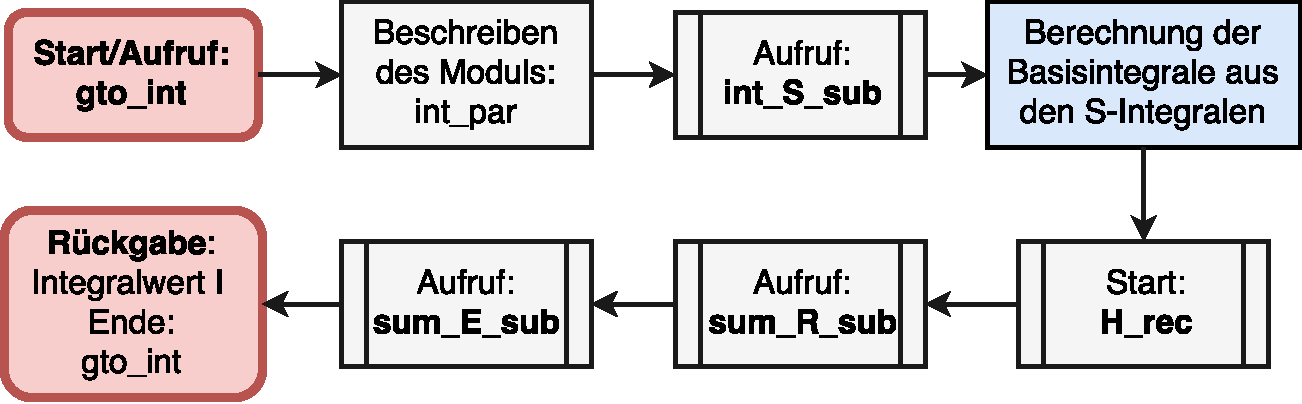
\includegraphics[scale=0.7]{gto_int.pdf}
	%	\vspace*{-10mm}
	\caption{Programmablaufplan der Subroutine \texttt{gto\_int}}
	\vspace{2mm} %\hrule 
	\label{pic:FC:gto_int} 
\end{figure}
%
Das Modul \texttt{int\_par} stellt eine Sammlung aller für das Integral 
wichtigen 
Parameter, wie zum Beispiel Exponenten der GTOs oder die erwähnten 
Potentialparameter\footnote{Der Programmteil des Beschreibens von 
\texttt{int\_par}, das 
Modul \texttt{int\_par} selbst und die Berechnung der Basisintegrale aus den 
S-Integralen
müsste angepasst werden, um weitere Potentialtypen hinzuzufügen.}, für alle 
weiteren Teilprogramme bereit. 
\texttt{int\_S\_sub}, \texttt{H\_rec}, \texttt{sum\_R\_sub} und 
\texttt{sum\_E\_sub} sind Teilprogramme, die im 
Folgenden noch näher beschrieben werden. Programmschritt 3 (Berechnung der 
Basisintegrale $\Pi_j^\pm$) wird je nach gewähltem Potential mit Formel 
\ref{eq:PIinS_MRP} bzw. \ref{eq:PI_LJP} durchgeführt.
%
%
%
\subsubsection{$S$ Integrale mit \texttt{int\_S\_sub}}
%
Einer der ersten Schritte ist die Berechnung der S-Integrale \ref{eq:def:S}. Je 
nach Potential kann $\alpha$ positiv, als auch negativ sein und so in das 
Renormierungschema \ref{sec:renorm} rutschen. Weiterhin muss immer eine Schar 
an Integralen berechnet werden, für jedes j der $\Pi^\pm_j$-Integrale. Daher 
wird \texttt{int\_S\_sub} derart designt, dass zu einem gegebenen maximalen j 
und 
gegebenen Potentialtyp ein Vektor aller benötigten S-Integrale ausgegeben wird.
Ausgehend vom Potentialtyp wird zunächst $\alpha$, mit der Obergrenze von j, 
$\beta$ und $\gamma$ berechnet. Weiterhin kann die Untergrenze (j=1) von 
$\alpha$ angegeben werden; diese Größe soll nun $\alpha_s$ heißen. Anschließend 
treten die Größen
\begin{align}\label{eq:def:parameter y,x}
y=\frac{\beta^2}{4 \gamma}= \xi Q^2 \quad\text{und}\quad 
x=\frac{\gamma}{\beta^2}=\frac{1}{4y}=\frac{1}{4\xi Q^2}
\end{align}
häufig auf und können gut zur Unterscheidung pathologischer Fälle genutzt 
werden.
%
\begin{figure}[H] \centering
	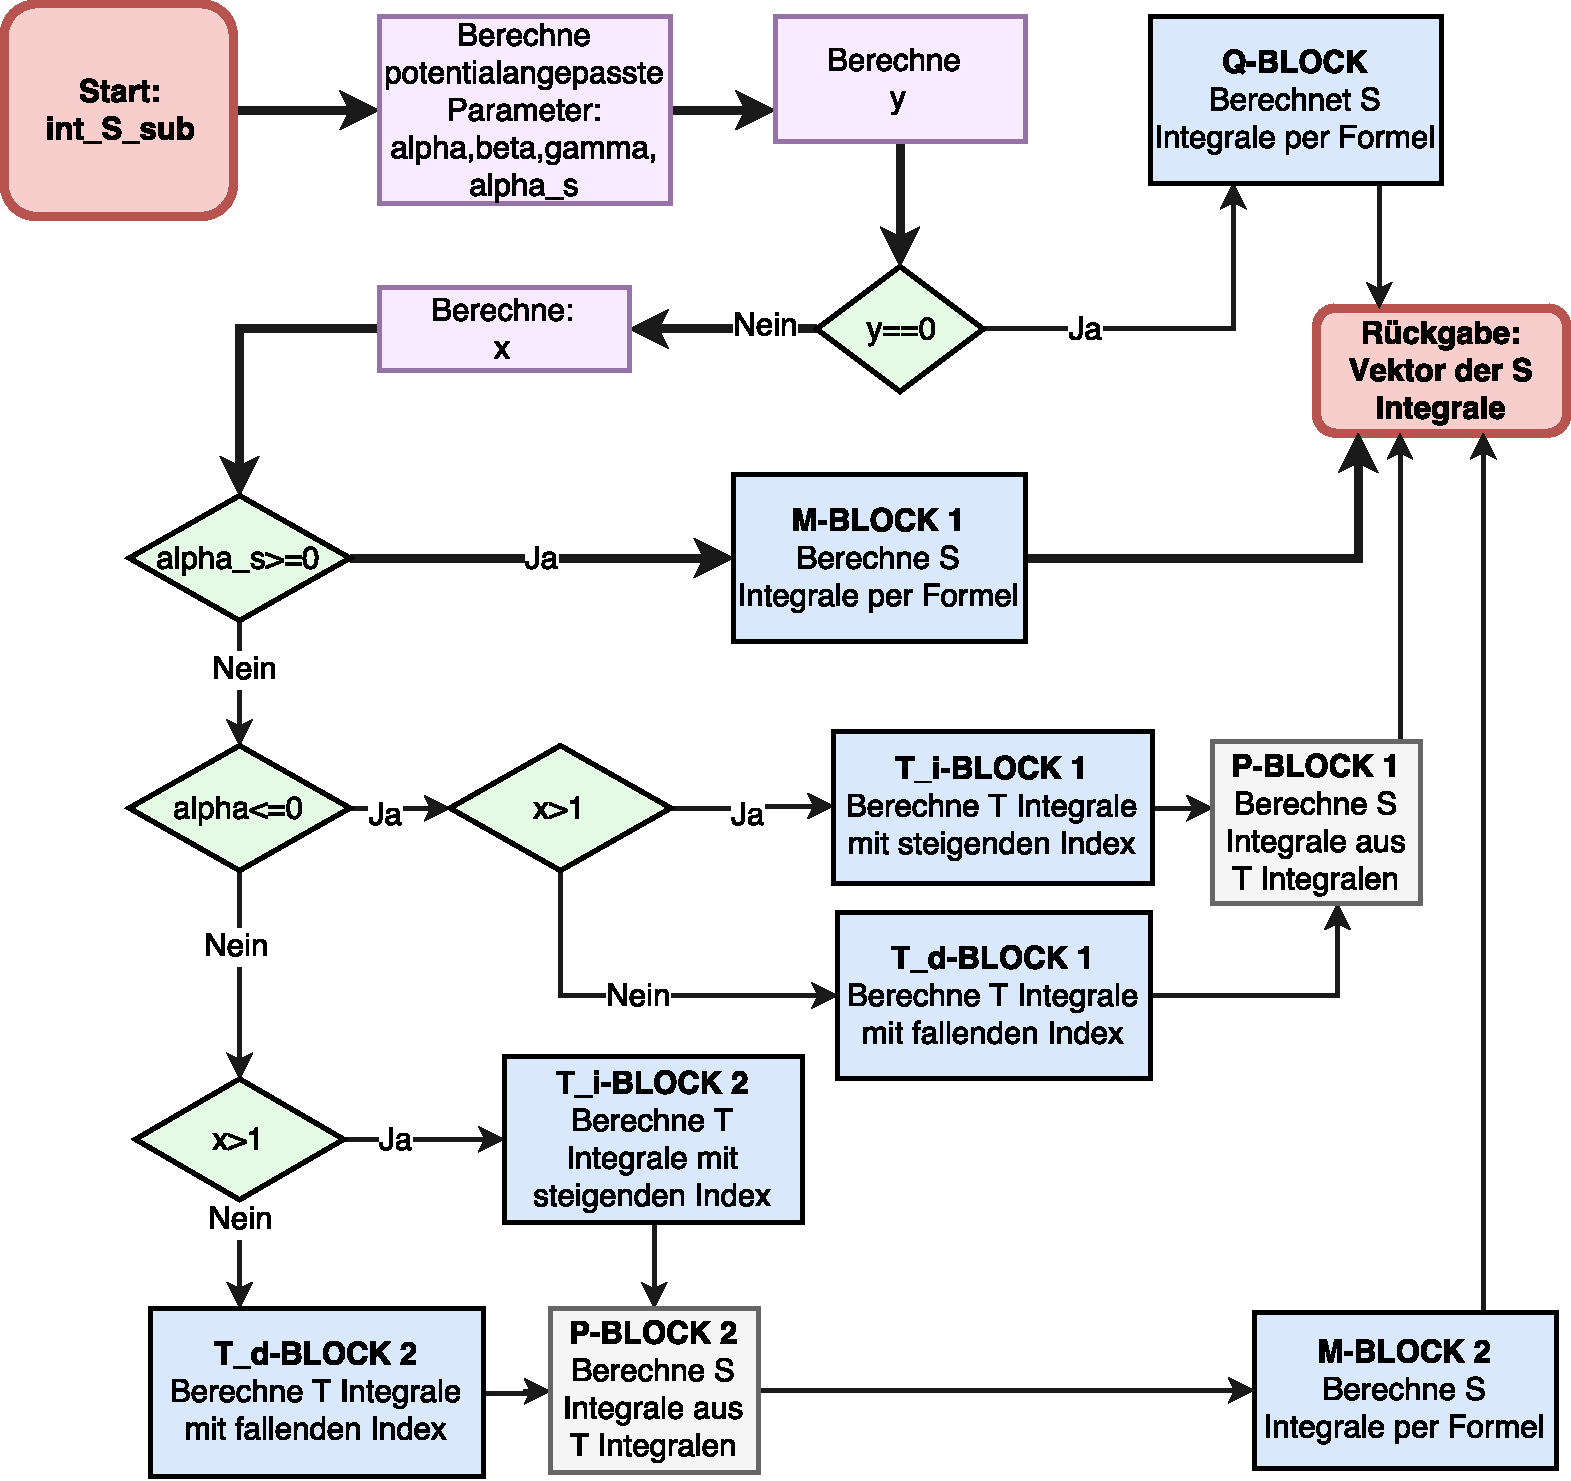
\includegraphics[scale=0.59]{int_S_sub.pdf}
	%	\vspace*{-10mm}
	\caption{Programmablaufplan der Subroutine \texttt{int\_S\_sub} zur 
	Berechnung der 
	Integrale \ref{eq:def:S} mit der Möglichkeit der Nutzung des 
	Renormierungschemas in Abschnitt \ref{sec:renorm}. Dick markiert ist der 
	Pfad ohne Nutzung einer Renormierung (Standard Pfad).}
	\vspace{2mm} %\hrule 
	\label{pic:FC:int_S_sub} 
\end{figure}
%TODO pagebreak in finaler version
%
Wie in Abbildung \ref{pic:FC:int_S_sub} zu sehen, enthält \texttt{int\_S\_sub} 
verschiedene Berechnungsblöcke. Folgende Auflistung beschreibt kurz ihren 
jeweiligen Zweck:
%
\begin{enumerate}
	\item \textbf{M-Block 1} berechnet für alle j die S-Integrale mithilfe der 
	Formel 
	\ref{eq:S,alpha>0}. Alle $\alpha(j)$ sind positiv, da $\alpha_s \geq0$ 
	(kein Renormierungsschema).
	%
	\item \textbf{M-Block 2} berechnet ein Teil der S-Integrale für alle j mit 
	$\alpha(j)>0$ mit Formel \ref{eq:S,alpha>0} (kein Renormierungsschema). 
	%
	\item \textbf{T\_i-Block 1/2} berechnen unter Zuhilfenahme des 
	Renormierungsschemas in \ref{sec:renorm} die T-Integrale \ref{eq:def:T-Int} 
	mit wachsenden Index $s=-\alpha(j)$ in der Rekursion \ref{eq:recursivT}.
	%
	\item \textbf{T\_d-Block 1/2} berechnet unter Zuhilfenahme des 
	Renormierungsschemas in \ref{sec:renorm} die T-Integrale \ref{eq:def:T-Int} 
	mit fallenden Index $s=-\alpha(j)$ in der Rekursion \ref{recursiveT2}.
	%
	\item \textbf{P-Block 1/2} berechnet die S-Integrale für negative $\alpha$ 
	aus den T-Integralen durch Formel \ref{eq:SinT}.
	%
	\item \textbf{Q-Block} berechnet S-Integrale für Q==0. Dadurch vereinfacht 
	sich das Integral enorm und kann fast ausschließlich durch Fakultäten 
	berechnet werden. Für negative $\alpha(j)$ wird das Renormierungsschema 
	\ref{sec:renorm} analytisch angewandt. Da für die Verwendung in 
	\texttt{gto\_int} Q 
	nie 0 sein wird, da hier der Algorithmus nicht funktioniert (siehe zum 
	Beispiel \ref{eq:Hobson}), werden die Formeln für diesen Block lediglich in 
	der Dokumentation stehen. Weiterhin sei erwähnt, dass dieser Block zur 
	Fehlerbehebung und der Vollständigkeit halber implementiert wird; 
	\texttt{int\_S\_sub} kann damit auch in anderen Programmen wiederverwendet 
	werden.
\end{enumerate}
%
Für das MRP und die Potentiale $V_1$ und $V_2$, welche keine Renormierung 
benötigen, wird nur der dick markierte Pfad verwendet.
%
%
%
\subsubsection{Rekursive Funktion \texttt{H\_rec} für $\mathcal{H}_{11l}^\pm$}
%
%
\begin{figure}[H] \centering
	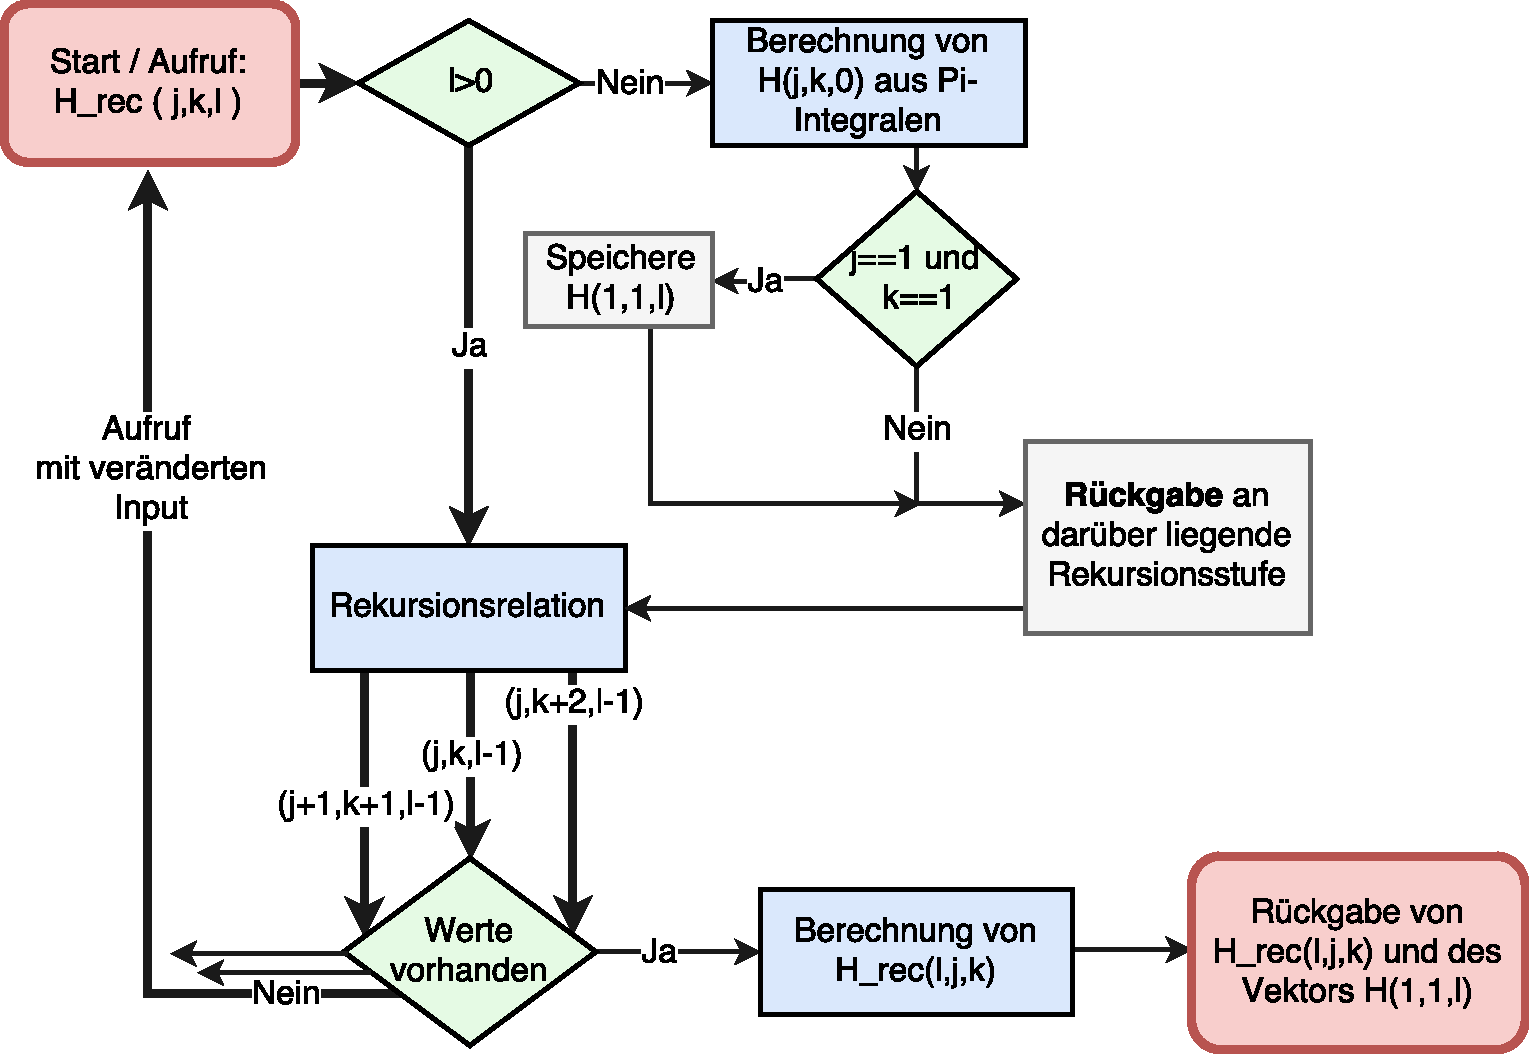
\includegraphics[scale=0.55]{H_rec.pdf}
	%\vspace*{-10mm}
	\caption{Programmablaufplan der rekursiven Funktion \texttt{H\_rec}  unter 
		Verwendung der Formeln \ref{eq:rek:H}  und \ref{eq:prop:H}. Pfade, die 
		auf 
		den Start zurückführen, bedeuten einen rekursiven Aufruf mit 
		veränderten 
		Input. Der dick markierte Pfad zeigt die Rekursionsschleife.}
	%\vspace{2mm} %\hrule 
	\label{pic:FC:H_rec} 
\end{figure}
%
Mithilfe der in \texttt{gto\_int} (unter Verwendung der S-Integrale) 
berechneten 
$\Pi^\pm_j$-Integralen wird nun die Rekursion \texttt{H\_rec} durchgeführt.
Die zentrale Formel hierbei ist die Rekursionsrelation \ref{eq:rek:H}.\\
%
 Abbildung 
\ref{pic:FC:H_rec} zeigt den konzeptionellen Ablauf der Funktion. Führt ein 
Pfad zurück auf das Startfeld, so bedeutet dies einen rekursiven 
Aufruf. Wird ein Ergebnis in der tiefsten Rekursionsstufe (l=0) berechnet, 
führt das zu einer Rückgabe des Werts an die Rekursionsrelation und damit zu 
einer Berechnung der darüber liegenden Stufe. Die Abfrage "Werte vorhanden"\ 
ist keine im Quellcode ersichtliche Programmstelle, sie veranschaulicht hier
lediglich die Funktionsweise eines rekursiven Aufrufs. Weiterhin wird darauf 
hingewiesen, dass diese Rekursion mit dem maximalen Indizes gestartet wird. Im 
Laufe der Rekursion werden dabei alle Fälle mit j=1 und k=1 mit beliebigen l in 
ein 
Vektor gespeichert. So kann sichergestellt werden, dass alle 
benötigten Werte für den nächsten Schritt (Formel \ref{R_sum}) bereit stehen. 
Zusätzlich ist in Abbildung \ref{pic:FC:H_rec} ersichtlich, dass bei jeder 
Rekursionsschleife drei 
Aufrufe der Funktion folgen. Da in jeder Stufe l um 1 reduziert wird, 
ergeben 
sich $3^l$ rekursive Aufrufe. l ergibt sich, wie in  Abschnitt über 
\ref{eq:final:Hobson} zu sehen, aus 
der Summe aller Potenzen der Monome der GTOs. Da in der Praxis 
selten höher als d-Orbitale betrachtet werden, sind Werte größer als $l=4\cdot 
(2+2+2)=24$ nicht 
zu erwarten. Dennoch ist die daraus resultierende Anzahl\footnote{für vier GTOs 
in 
d-Orbitalen, dh. l=24 folgen $3^{24}=282429536481\approx3\cdot 10^{11}$ 
rekursive Aufrufe der Funktion \texttt{H\_rec}} der Funktionsaufrufe sehr 
hoch und kann prinzipiell zu Fehlern führen. Daher wird an dieser Stelle auf 
potentielle Laufzeitprobleme oder Rundungsfehler für hohe Orbitale hingewiesen.
%
%
%
\subsubsection{Subroutine \texttt{sum\_R\_sub}}
%
Die Subroutine \texttt{sum\_R\_sub} soll nun alle relevanten kartesischen 
Ableitungen des Basisintegrals unter Anwendung des Hobson Theorems berechnen. 
Die schon in Kapitel 
\ref{sec:Algorithmus} dargelegte Formel \ref{R_sum} 
führt diesen Schritt auf eine Summe über die radialen Ableitungen 
$\mathcal{H}_{11l}$ zurück. Eine erste Optimierung dieser Berechnung zeigt 
sich, wenn auf die richtige Berechnungsreihenfolge der Summen geachtet wird. 
Die m-Summe 
und die k-Summe sind unabhängig voneinander und müssen somit nicht 
geschachtelt berechnet werden. Es gilt also
%
\begin{align}\nonumber
R^{\tau,\rho,\sigma}&=\sum_{l=0}^{l_{max}} 
%
\underset{=:R_m(\,l\,;\,c^{-1},Z)}{\underbrace{\sum_{m=-l}^{l}c^{-1}(l,m,\tau,\rho,\sigma)Z_{lm}(\textbf{Q})}}
%
\underset{=:R_k(l\, ;\, 
\mathcal{H}^\pm_{11l},d,Q)}{\underbrace{\sum_{k=0}^{k_{max}}d_k^{l,k_{max}} 
\cdot 
\left[(\mathcal{H}^-_{11l}-\mathcal{H}^+_{11l})\right]Q^{l_{max}-l-2k}}}\\\label{eq:short_R_sum}
%
&=\sum_{l=0}^{l_{max}}R_m(l)\cdot R_k(l)\qquad,
\end{align}
%
wobei ($\tau,\rho,\sigma$) für alle möglichen  Kombinationen der Potenzen der 
Ableitungen stehen. Die maximalen Werte können an Gleichung \ref{eq:E:Koef} 
abgelesen werden.\\
Für die Implementierung ist weiterhin wichtig:
\begin{enumerate}
	\item alle Werte von ($\tau,\rho,\sigma$) abzulaufen (die ersten "drei"\  
	Schleifen, die mit den Indizes t,u,v gekennzeichnet sind, vlg. 
	\ref{eq:E:Koef} bzw. Abbildung \ref{pic:FC:sum_R_sub}).
	%
	\item die im Abschnitt \ref{sec:Hobson_schlegel} 
	erwähnte, aus \cite{av:9a} stammende Bedingung, dass $c^{-1}\equiv0$ ist, 
	falls $l-l_{max}$ ungerade wird, zu berücksichtigen.
	\item die zwei unabhängigen Summen $R_m(l)$ und $R_k(l)$ separat und nicht 
	geschachtelt zu berechnen.
	\item d und $c^{-1}$ Koeffizienten möglichst außerhalb der 
	Schleifenstruktur vorher zu berechnen, um Funktionsaufrufe zu minimieren. 
\end{enumerate}
%
\begin{figure}[H] \centering
	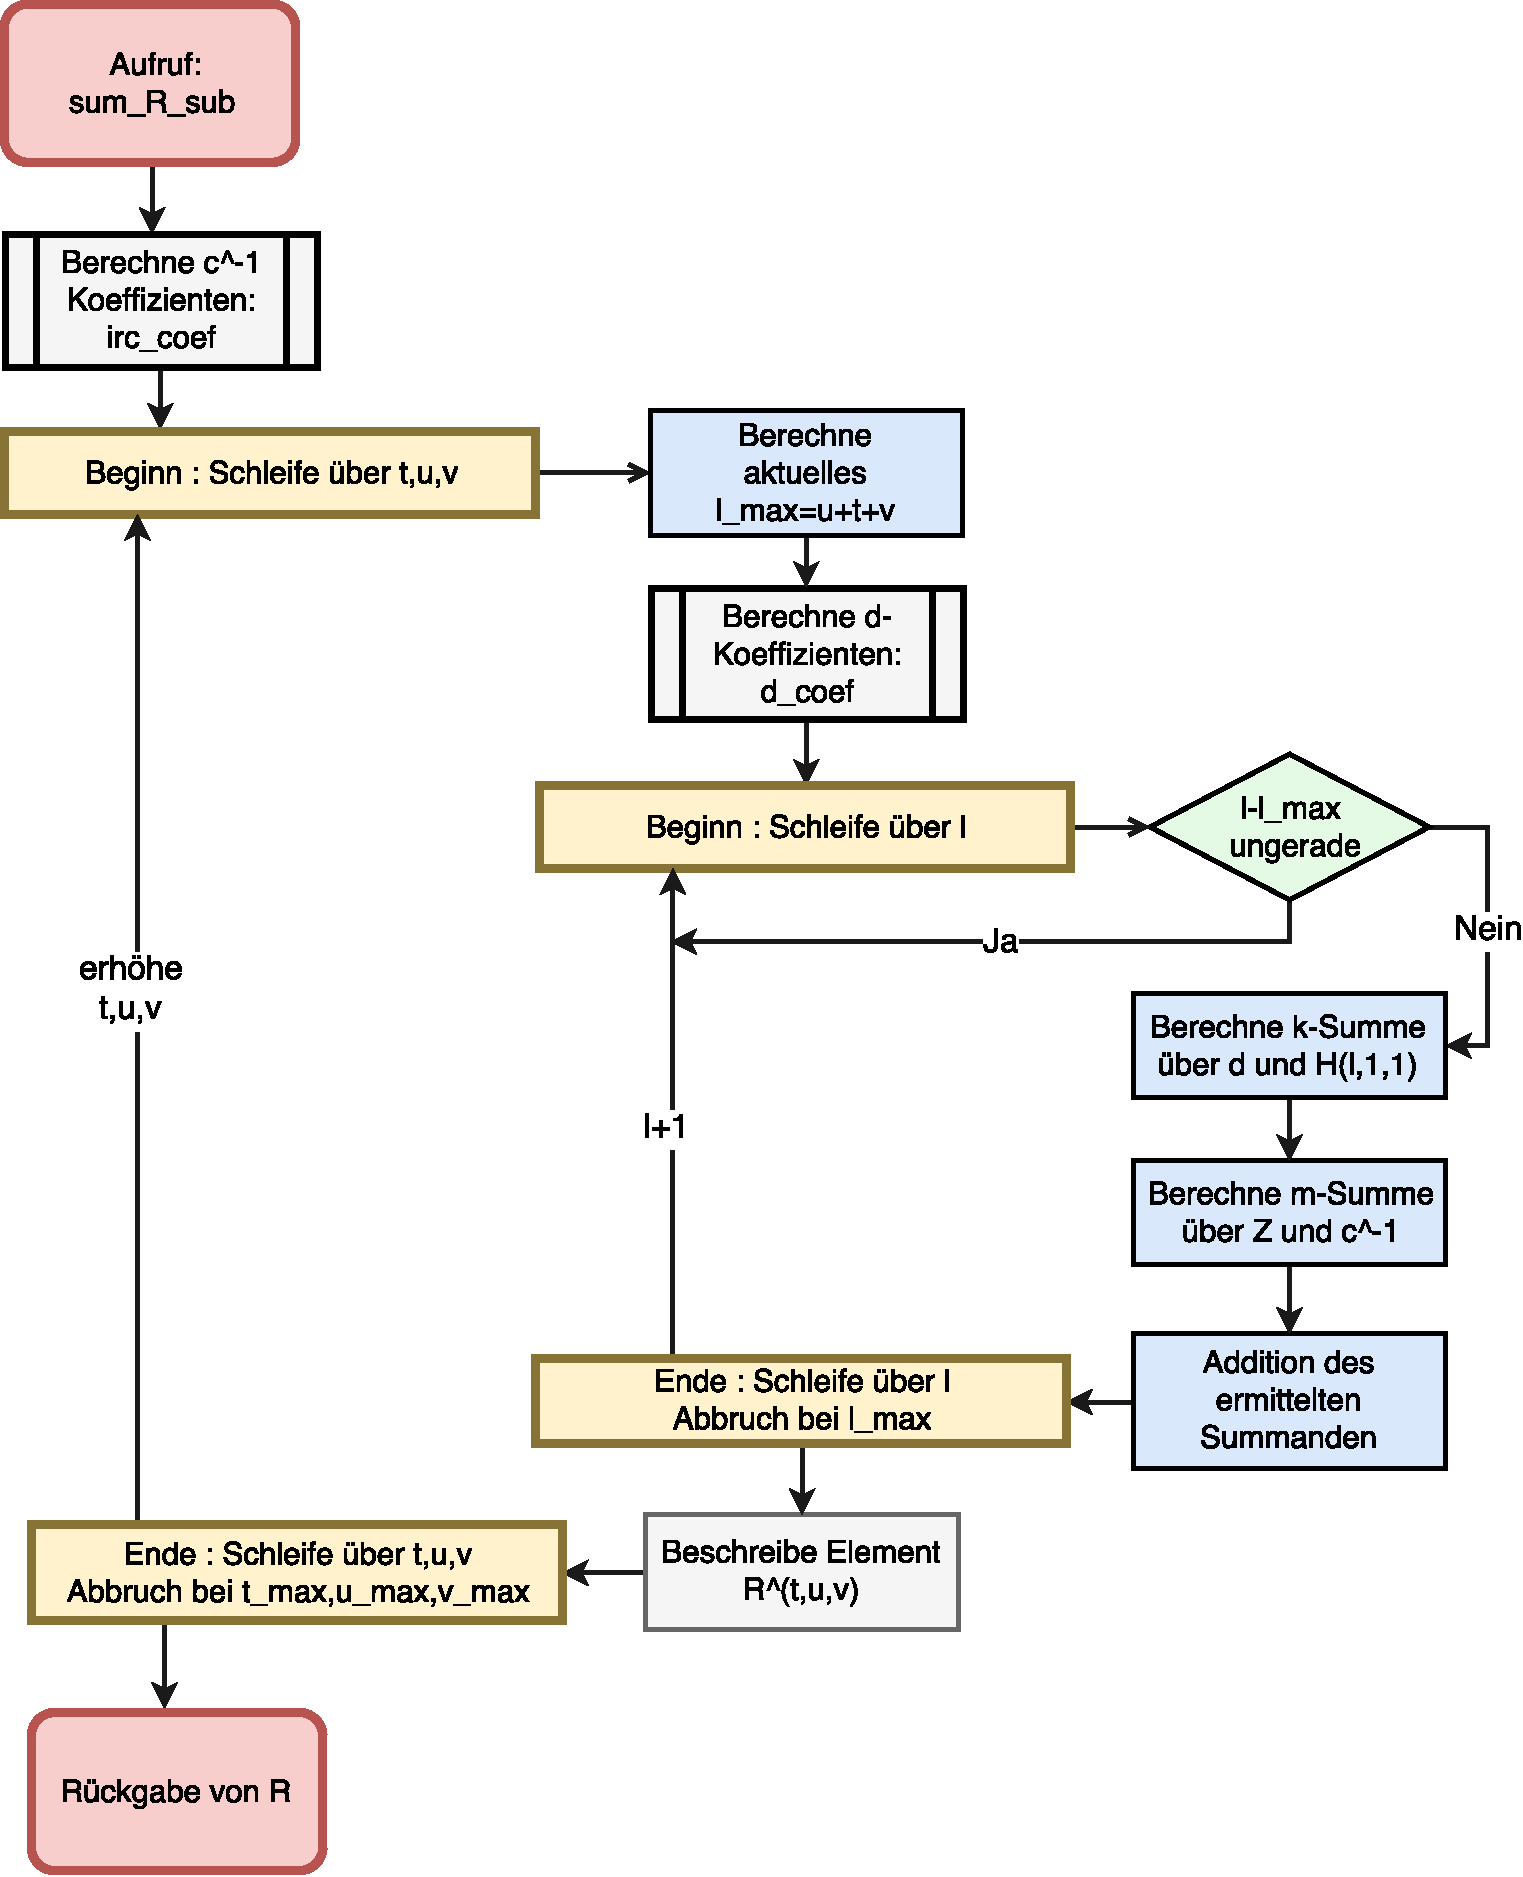
\includegraphics[scale=0.6]{sum_R_sub.pdf}
	%\vspace*{-10mm}
	\caption{Programmablaufplan der Subroutine 
	\texttt{sum\_R\_sub}. 1. Schleife geht über alle 
	Einträge von R, die 2. Schleife summiert über l 
	vlg. Formel \ref{eq:short_R_sum}. Die Summen über k 
	und m sind in den blauen 
	Blöcken rechts zusammengefasst.}
	%\vspace{2mm} %\hrule 
	\label{pic:FC:sum_R_sub} 
\end{figure}
%
Zurückgegeben wird ein 3d-Feld $R^{\tau,\rho,\sigma}$, 
welches in der Routine \texttt{sum\_E\_sub} wiederverwendet 
wird. Bevor diese erläutert wird, 
sollen kurz die Subroutinen zur Berechnung der Koeffizienten skizziert werden.
%
\subparagraph{Zur Berechnung der d-Koeffizienten mit \texttt{d\_coef}}
%
wird Formel \ref{eq:rek_d} benutzt. $d^{l,k_{max}}_{k}$ hat drei freie 
Parameter; sobald $l_{max}$ festgelegt ist (vgl. 
Abbildung 
\ref{pic:FC:sum_R_sub} ), kann d als Matrix der 
Ausdehnung $l_{max}\times k_{max}$ aufgefasst werden. Die 
Subroutine geht dabei folgende Schritte durch:
\begin{enumerate}
	\item Gehe alle möglichen Zahlen für l und k durch.
	\item Starte für die gegebene Kombination von l, k die Rekursion 
	\ref{eq:rek_d} , welche durch die Funktion \texttt{d\_rec} realisiert ist.
	\item Speichere das Ergebnis in der Matrix d(k,l).
\end{enumerate} 
Diese Matrix wird anschließend an \texttt{sum\_R\_sub} zurückgegeben. 
%
%
%
\subparagraph{Die Berechnung der $c^{-1}$-Koeffizienten mit \texttt{irc\_coef}}
%
benutzt in erster Linie die Gleichung \ref{eq:def:c_koef}. Zu erkennen ist 
jedoch, dass dazu die c-Koeffizienten benötigt werden. Die Formel für diese 
wird der Arbeit \cite{av:4a} entnommen, wobei jedoch auch hier kleinere 
Tippfehler vorhanden sind. Im Anhang \ref{sec:AnhangA:Schlegel} sind alle 
benötigten Formeln bzgl. c und der damit verbundenen Transformation richtig 
gestellt und angegeben.  Weiterhin sind dort noch weitere Anmerkungen zur 
Implementierung vorhanden. %(??)
%
%
%
\subsubsection{Subroutine \texttt{sum\_E\_sub}}
%
Nachdem nun das Feld $R^{\tau,\rho,\sigma}$ bekannt ist, muss die Summe 
\ref{eq:E:Koef}\  ausgeführt werden. Diese Summe wird durch die Subroutine 
\texttt{sum\_E\_sub} durchgeführt. Dazu werden die oben erwähnten Koeffizienten 
$E^{ij}_t$ (\ref{eq:E:coef1} - \ref{eq:E:coef4}) benötigt, welche mit der 
Subroutine \texttt{E\_coef} berechnet werden. Hier werden für gegebene Zahlen i 
und j 
alle t durchgegangen und anschließend die Rekursionen ab \ref{eq:E:coef4} 
gestartet. Diese Rekursionen sind in der Funktion \texttt{E\_rec} 
implementiert. Dabei 
unterscheidet \texttt{E\_rec} folgende Fälle:
\begin{enumerate}
	\item i=j=t=0 $\Rightarrow$ Gleichung \ref{eq:E:coef1}
	\item i,j,t < 0 oder t>i+j $\Rightarrow$ $E^{ij}_t=0$
	\item $t\neq0$ $\Rightarrow$ Gleichung \ref{eq:E:coef4}
	\item $t=0$ und $i\neq0$ $\Rightarrow$ Gleichung \ref{eq:E:coef2}
	\item $t=0$ und $i=0$ und $j\neq0$ $\Rightarrow$ Gleichung \ref{eq:E:coef3}
\end{enumerate}
Wobei \ref{eq:E:coef2} und \ref{eq:E:coef3} auf abfallende Index, das heißt 
$E^{i,j}_t(i-1,j,t)$,  umgeschrieben sind.   \\
Nachdem alle Koeffizienten bekannt sind, muss nun die Summe \ref{eq:E:Koef} 
ausgeführt werden. Diese wird durch 6 ineinander geschachtelte Schleifen 
realisiert. 
%
%
%
\subsubsection{Weitere mathematische Funktionen}
%
Neben den schon diskutierten Funktionen und Subroutinen werden noch einige 
kleinere mathematische Funktionen benötigt, um alle Rechnungen durchzuführen.  
\begin{enumerate}
	\item In \texttt{int\_S\_sub}, genauer in den T-Blöcken, muss im Rahmen des 
	Renormierungsschemas die Funktionen $\omega_1(x)$, $\omega_0(x)$ und die 
	Diagamma-Funktion $\psi_d$ für ganz und halbzahlige Integer ausgewertet 
	werden. Diese werden in den Funktionen  \texttt{w1}, \texttt{w0} und 
	\texttt{diagamm} realisiert und folgen im Wesentlichen der 
	Berechnungsmethode aus \cite{av:1a2} für positive x. Im Anhang 
	\ref{sec:AnhangB:T_Integral} sind die entscheidenen Formeln für die 
	Berechnung gegeben.
	\item Weiterhin wird in \texttt{int\_S\_sub} (in den M-Blöcken) die 
	konfluierte hypergeometrische Funktion M berechnet. Die entsprechende 
	Realisierung der Reihendarstellung \ref{eq:reihe_M_kon.hyp.geo} unter 
	Verwendung der Pochhammer-Symbole ist in den Funktionen 
	\texttt{con\_hyp\_geo\_M} und \texttt{PHS} bewerkstelligt.
	\item In \texttt{sum\_R\_sub} werden die reellen soliden 
	Kugelflächenfunktionen benutzt. Die Berechnung dieser läuft über die 
	assoziierten Legendrepolynome, die durch die Routine \texttt{plgndr} aus 
	\cite{b:4a} berechnet werden. Restliche Konstanten, Fallunterscheidungen, 
	der Radial- und der $\phi$-Anteil werden in der Funktion \texttt{rsSHS} 
	bearbeitet. Nötige Definitionen und Konversionen sind im Anhang 
	\ref{sec:AnhangA:Schlegel} angegeben. 
    \item Allgemein werden Binomialkoeffizienten und Fakultäten benötigt. Dafür 
    benutzt man in erster Linie die Routinen \texttt{factrl} und \texttt{bico} 
    aus 
    \cite{b:4a}. Hinzu kommt die Funktion \texttt{cfact}, welche eine 
    Berechnung  eines Bruches von Fakultäten gekürzt berechnet 
    ($\frac{10!}{8!}=10\cdot 9$).
\end{enumerate}
%
%
%
\section{Genauigkeitstests}
%
In diesem Abschnitt soll auf verschiedene Weisen die Genauigkeit des Programms 
getestet werden. Dazu wird unter anderem eine Subroutine der NAG Bibliothek 
genutzt. Unter \cite{o:1a} kann die Dokumentation der genutzten Routine 
\texttt{D01FCF} 
abgerufen werden. \texttt{D01FCF} ist in der Arbeitsgruppe verfügbar und löst 
das 
sechsdimensionale Integral durch adaptive Quadratur über Hyperrechtecke. Die 
im Folgenden verwendete Größe ACC gibt die intern geschätzte Genauigkeit der 
NAG-Routine an. Weiterhin sei darauf hingewiesen, dass 
sich sprachlich auch in diesem Abschnitt auf die 
physikalische Gegebenheit bezogen wird, aber keinerlei 
Einheiten angegeben werden, da es sich dennoch um eine 
rein mathematische Betrachtung handelt. So wird zum 
Beispiel der später zu variierende Parameter $A_x$ als 
Abstand bezeichnet, um so die Benennung/ Unterscheidung zu 
vereinfachen und den späteren Bezug zur Physik nicht zu 
vergessen.
%
%
%
\subsection{Normberechnung ($f_{12}\equiv 1$)}\label{sec:T:norm}
%
Der erste Test den man an dem Programm durchführen kann, ist das 
Wechselwirkungspotential 1 zu setzen. Für nicht normierte GTOs ergibt sich 
mit dem Potential \ref{eq:def:V1} :  $f_{12}=V_1=1$ :
%
\begin{align*}
I&=\int\int\ d\textbf{r}_1\ d\textbf{r}_2 
(\psi_i^a(\textbf{r}_1)\psi_i^c(\textbf{r}_2))^*\cdot  1 \cdot  
\psi_j^b(\textbf{r}_1)\psi_j^d(\textbf{r}_2)\\
& =\int\ d\textbf{r}_1  \cdot 
x_{1,A}^i\,y_{1,A}^k\,z_{1,A}^m\cdot  
x_{1,B}^j\,y_{1,B}^l\,z_{1,B}^n\cdot e^{-b r_{1,B}^2-a 
	r_{1,A}^2} \cdot \\
&\qquad  \cdot \int\ d\textbf{r}_2\   
x_{2,C}^{i'}\,y_{2,C}^{k'}\,z_{2,C}^{m'} \cdot  
x_{2,D}^{j'}\,y_{2,D}^{l'}\,z_{2,D}^{n'}\cdot e^{-c r_{2,C}^2-d 
	r_{2,D}^2}\qquad.%\\
%&= N_{ikm}(a)N_{jln}(b)N_{i'k'm'}(c)N_{j'l'n'}(d) \qquad.
\end{align*}
%
Einfachheitshalber wird außerdem angenommen, dass 
%
\begin{align}\nonumber
\textbf{A}=\textbf{B} \quad&,\quad 
\textbf{C}=\textbf{D}\\\nonumber
a=b \quad&,\quad c=d\\\label{eq:tests:annahmen:norm}
(i,k,m)=(j,l,n) \quad&,\quad (i',k',m')=(j',l',n')
\end{align}
%
gilt. Damit wird das Integral zu
\begin{align}\label{eq:I_NORM}
I=I_\text{Norm}=N_{ikm}(a)^2 \cdot N_{i'k'm'}(c)^2 
\quad.
\end{align}
%
Diese Normen können durch die Formel \ref{eq:NORM} berechnet werden und stellen 
somit eine gute Überprüfungsmehtode dar. Die Berechnung 
beinhaltet weder 
kritische Summen noch relevante Funktionsaufrufe, die die Genauigkeit 
verschlechtern  könnten; das Ergebnis wird als wesentlich genauer als alle 
anderen Berechnungsmethoden angesehen.
%
\subsubsection{Variation des Orbitals}
%
Im Folgenden wird $(i',k',m')=(0,0,0)$ 
gesetzt und $(i,k,m)$ variiert. Es sei gesagt, dass der vertauschte Fall auch 
getestet wird und zu vergleichbaren Ergebnissen führt.  Weiterhin wird auf die 
Größe $l=2\cdot (i+k+m) $ hingewiesen. Die 2 entsteht durch die 
gegebenen Annahmen; allgemein ist l die Summe über alle Potenzen der GTOs. l 
gibt damit eine Charakteristik der Komplexität des Integrals an. 
Dementsprechend zeigen auch die folgenden Tests für unterschiedliche Orbitale 
mit gleichem l gleiche oder sogar höhere 
Genauigkeiten\footnote{Siehe dazu speziell die Orbitale 
(1,0,2) und (1,1,1) in Tabelle 
\ref{tab:norm:orbital}.}. Tabelle 
\ref{tab:norm:orbital} zeigt 
eine Auswahl der Testergebnisse, bei denen $A_x=1$, alle anderen Komponenten 0, 
\textbf{C}=\textbf{0} und a=c=0,001 konstant gesetzt worden ist.
%
\begin{table}[H] \centering
	\caption{Genauigkeitstest der Subroutine \texttt{gto\_int} 
	zu 
	verschiedenen 
	Orbitalen durch Normberechnung im Vergleich zu 
	analytischen Ergebnissen und 
	der numerischen NAG-Berechnung mit $A_x=1$ und 
	a=c=0,001.} \vspace{0.2cm}
	\begin{threeparttable} 
		\begin{tabular}{c|c||c||c||c}
			l&Orbital&  $I_\text{gto\_int}$            
			&  $I_\text{Norm}$     
			&$\left|\frac{I_\text{gto\_int}-I_\text{Norm}}{I_\text{Norm}}\right|$
			 \\ \hline\hline
			0&(0,0,0)&3,87578458503748E+09 & 
			3,87578458503748E+09 & 9,84E-16 \\
			2&(1,0,0)&9,68946146260323E+11 & 
			9,68946146259369E+11 & 9,85E-13 \\
			4&(0,0,2)&7,26709609873341E+14 & 
			7,26709609694527E+14 & 2,46E-10 \\
			6&(1,0,2)&1,81677760185790E+17 & 
			1,81677402423632E+17 & 1,97E-06 \\
			6&(1,1,1)&6,05592533952633E+16 &
			6,05591341412106E+16 & 1,97E-06 \\
			8&(2,0,2)&1,33465693978348E+20 & 
			1,36258051817724E+20 & 2,05E-02 
		\end{tabular}
		\vspace{4mm}
		\begin{tabular}{c|c||c||c|c||c}
			l&Orbital&  $I_\text{gto\_int}$ & 
			$I_\text{NAG}$           & ACC 
			[\%] & 
			$\left|\frac{I_\text{gto\_int}-I_\text{NAG}}{I_\text{gto\_int}}\right|$
			 \\ \hline\hline
			0&(0,0,0)&3,87578458503748E+09& 
			3,8757824E+09 & 3,87E-05 & 5,48E-07 
			\\
			2&(1,0,0)&9,68946146260323E+11& 
			9,6892021E+11 & 6,81E-05 & 2,67E-05 
			\\
			4&(0,0,2)&7,26709609873341E+14& 
			7,2670508E+14 & 8,91E-05 & 6,22E-06 
			\\
			6&(1,0,2)&1,81677760185790E+17& 
			1,8166964E+17 & 2,31E-04 & 4,47E-05 
		\end{tabular}
%		\begin{tablenotes}
		%	\item[I] 
%		\end{tablenotes}
	\end{threeparttable}
	\label{tab:norm:orbital}
\end{table}
%

In der Tabelle \ref{tab:norm:orbital} ist zu sehen, dass \texttt{gto\_int}, die 
NAG-Routine und die analytischen 
Berechnungen nach Formel \ref{eq:I_NORM} mithilfe der Norm vergleichbare Werte 
liefern. Das heißt, dass der Algorithmus prinzipiell funktioniert und die 
Implementierung in den hier gezeigten Fällen richtig ist. Im Vergleich zu der 
analytischen Berechnung zeigt sich, dass sich die relative Abweichung für ein 
höheres Orbital um 3-4 Größenordnungen verschlechtert. Zurückzuführen kann 
dieser Genauigkeitsverlust zum einen auf die Berechnung des Basisintegrals und 
zum anderen auf Rundungsfehler. Im Implementierungsstadium wird beobachtet, 
dass ein Basisintegral mit einem Fehler im wenigen Prozentbereich eine 
Ungenauigkeit von 6 Größenordnungen für das Integral mit sich führt, das heißt, 
dass dadurch
ein vollkommen falsches Ergebnis entsteht. Daher ist der Algorithmus sehr 
sensitiv auf Ungenauigkeiten des Basisintegrals. Dementsprechend kann 
vermutlich die Genauigkeit weiter erhöht werden, indem die Berechnung das 
Basisintegrals verbessert wird. Es soll daher erörtert werden, wie der in 
\cite{av:1a} und \cite{av:1a2} dargestellte Berechnungsweg von S ( Definition 
\ref{eq:def:S}) mithilfe der Tricomis konfluierten hypergeometrischen Funktion 
$\mathcal{U}$ korrigiert werden muss, um auch diesen verwenden zu können. 
Vorteil der dort dargestellten Berechnungsmethode ist, dass für 
unterschiedliche 
Intervalle der Eingabeparameter auch andere Berechnungsmethoden verwendet 
werden und so für 
einen größeren Bereich das Ergebnis die Genauigkeit beibehält. Im 
Falle von Rundungsfehlern bzw. Fehler, die durch 
Subtraktion zweier fast gleichgroßer Zahlen 
entstehen\footnote{z.B. in Formel \ref{eq:S,alpha>0} oder \ref{R_sum}
möglich}, 
kann untersucht werden, in welchem Programmteil diese 
aufkommen. Dafür nutzt man 
eine schon implementierte Debug-Funktion\footnote{Die Verwendung der 
detaillierten Ausgabe ist in der Dokumention erklärt.} im Programm. Im 
verantwortlichen Programmteil kann anschließend ein genauerer / 
höherer Datentyp (z.B. \texttt{REAL(KIND=16)} ) verwendet werden, um die 
Gesamtgenauigkeit zu erhöhen bzw. den Verlust von 
signifikanten Stellen zu verkleinern.\\

Weiterhin zeigt sich, dass im Vergleich zur NAG-Routine \texttt{gto\_int} ein 
vergleichbares bzw. besseres Ergebnis bis einschließlich l=6 erzeugt wird. Für 
l$\geq$8 soll \texttt{gto\_int} nicht mehr verwendet werden, 
da dort das Ergebnis kein Bezug mehr zum analytischen 
Ergebnis zeigt. Unter der Annahme, dass 
im Regime der ultrakalten Gase nur die einfachsten 
Orbitale eine Rolle spielen, 
kann man sich vorstellen, dass auch schon diese Stufe 
der Genauigkeit für die CI Rechnung 
ausreichen könnte. 

Die NAG-Routine hat unabhängig von l eine Genauigkeit 
von ungefähr $10^{-5}$ und kann nicht weiter gesteigert 
werden. Daher wird in diesem Abschnitt davon abgesehen, 
erneut mit der NAG-Routine zu vergleichen, da das 
analytische Ergebnis deutlich genauer ist.
%
\begin{table}[H] \centering
	\caption{Laufzeiten von \texttt{gto\_int} zu verschiedenen 
	Orbitalen. Es werden über 1000 Durchläufe 
	gemittelt.} \vspace{0.2cm}
	\begin{threeparttable} 
		\begin{tabular}{c|c||c}
		l&Orbital&Laufzeit [ms]\\ \hline
		0&(0,0,0)& 0,004\\
		2&(0,0,1)& 0,028\\
		2&(1,0,0)& 0,024\\
		4&(0,0,2)& 0,140\\
		6&(1,0,2)& 1,056\\
		8&(2,0,2)& 4,424\\
		10&(2,1,2)& 27,468\\
		12&(2,2,2)& 103,768\\
		\end{tabular}
		%		\begin{tablenotes}
		%	\item[I] 
		%		\end{tablenotes}
	\end{threeparttable}
	\label{tab:norm:orbital_time}
\end{table}
% 
Tabelle \ref{tab:norm:orbital_time} stellt Laufzeiten  
zu ihren Orbitalen dar. Dabei ist zu sehen, dass für 
ein höheres Orbital fast immer eine Größenordnung 
längerer Laufzeit benötigt wird. Für die sehr genau 
berechenbaren Integrale (l=\{0,2,4\}) werden nur rund 
0,2 ms benötigt, das heißt, es wären min. 5000 Integrale pro 
Sekunde möglich. Im Vergleich zu der NAG-Routine, die 
zwischen 87,404 s bis 93,052 s abhängig von l benötigt, 
ist \texttt{gto\_int} bis zu 5 Größenordnungen schneller. 
%
%
%
\subsubsection{Variation des Abstandes} 
\label{sec:var.Abstand_norm}
%
Nun soll das Orbital und die Exponenten konstant gehalten und der 
Abstand variiert werden. Die oben gewählten Annahmen 
\ref{eq:tests:annahmen:norm} bleiben weiterhin 
bestehen. An dieser Stelle sei nochmal darauf hingewiesen, dass der Algorithmus 
und damit das Programm nur für $Q\neq0$, das heißt für z.B.  
\textbf{A}=\textbf{B}$\neq$\textbf{C}=\textbf{D} funktioniert. 
(??) Dieser Fall entspricht einem Überlappintegral zwischen Orbitalen des 
selben 
Atoms oder zweier Orbitale von zwei Teilchen am selben Ort, was beides nicht 
vorkommen dürfte und daher auch nicht in dieser Arbeit betrachtet wird. \\
In diesem Test wird das Orbital $(i,k,m)=(1,0,0)$ und 
$(i',k',m')=(0,0,0)$ untersucht, da dieses ein 
repräsentatives, nicht triviales, aber dennoch sehr 
genaues zu berechnendes  Integral 
darstellt. Tabelle \ref{tab:norm:abstände} zeigt Ergebnisse von 
\texttt{gto\_int} zu 
verschiedenen Abständen der Teilchen ($\hat{=}$ Zentren der GTOs) im 
Vergleich zur analytischen Lösung durch Formel \ref{eq:I_NORM} zum konstanten 
Exponenten a=c=0,001 und zweiten Zentrum \textbf{C}=\textbf{0}.
%
\begin{table}[H] \centering
	\caption{Genauigkeitstest der Subroutine \texttt{gto\_int} 
	zu verschiedenen 
		Zentren der GTOs durch Normberechnung im Vergleich zu analytischen 
		Ergebnissen am Beispiel des (1,0,0)-Orbitals. 
		Eine kleinschrittigere Tabelle ist im Anhang 
		\ref{sec:AnhangC:Tests} gegeben.} \vspace{0.2cm}
	\begin{threeparttable} 
		\begin{tabular}{c||c||c||c}
			$A_x$&  $I_\text{gto\_int}$            &  $I_\text{Norm}$     
			&$\left|\frac{I_\text{gto\_int}-I_\text{Norm}}{I_\text{Norm}}\right|$
			\\ \hline\hline
			1   & 9,68946146260324E+11 & 9,68946146259369E+11 & 9,85E-13 \\
			101 & 9,68946146259356E+11 & 9,68946146259369E+11 & 1,36E-14 \\
			201 & 9,68946146311261E+11 & 9,68946146259369E+11 & 5,36E-11 \\
			271 & 8,2167349128430E+11 & 
			9,68946146311261E+11 & 1,52E-01\\
		\end{tabular}
		%		\begin{tablenotes}
		%	\item[I] 
		%		\end{tablenotes}
	\end{threeparttable}
	\label{tab:norm:abstände}
\end{table}
%
Zu sehen ist, 
dass offensichtlich die Norm unabhängig vom Abstand ist, da über den ganzen 
Raum integriert werden soll. Weiterhin ist ersichtlich, dass die Genauigkeit 
mit steigendem Abstand fällt. Zwischen Q=$A_x$=201  und 
271 fällt die 
Genauigkeit auf rund 15\% ab und ist damit für eine 
möglichst genaue Berechnung 
nicht mehr zu gebrauchen. Für noch größere Abstände hat 
das Ergebnis kaum noch einen Bezug zum richtigen 
Ergebnis.\\
Dieser Genauigkeitsverlust 
ist durch die Genauigkeit des Basisintegrals begründet. Die verwendete 
Reihendarstellung der Krummers konfluierten hypergeometrischen Funktion 
\ref{eq:reihe_M_kon.hyp.geo} konvergiert ab ungefähr $A_x$=201 nicht mehr 
vollständig 
(es wird 
eine Warnung vom Programm ausgegeben) und liefert damit nur eine 
Näherungslösung. Will man auch hier die Genauigkeit erhöhen, soll, wie beim 
Test der Orbitale erwähnt, eine bessere Berechnungsmethode für das 
Basisintegral gefunden werden. Der schnelle Genauigkeitsverlust kann durch die 
starke Sensibilität des Algorithmus auf das 
Basisintegral zurückgeführt werden. \\

Dieses Verhalten wird auch bei der Untersuchung der 
Laufzeit festgestellt. Grafik 
\ref{pic:test_norm_abstand_laufzeit} zeigt die Laufzeit 
des Programms in Abhängigkeit des Abstandes. Der 
Verlauf kann in drei Bereiche unterteilt werden. Für 
sehr kleine Abstände scheint die Laufzeit, konstant zu 
bleiben. Anschließend gibt es einen fast linearen 
Anstieg, der abrupt in ein leicht absteigendes Plateau 
übergeht. Diese Bereiche entsprechen dem Verhalten der 
Reihenentwicklung \ref{eq:reihe_M_kon.hyp.geo}. Für 
kleine Abstände konvergiert die Reihe schnell und 
andere Programmteile legen die Laufzeit fest. 
Anschließend benötigt die Reihe immer mehr Terme, um zu 
konvergieren / die geforderte Genauigkeit zu erreichen. 
Abschließend bricht die Reihe ab, da entweder eine nicht 
auswertbare Zahl entstanden ist (\texttt{NaN} oder \texttt{Inf}, dann wird das 
Ergebnis der Reihe 
ohne den nicht auswertbaren Term genutzt), der 
Wert für einige Glieder stagniert oder die maximale 
Anzahl der Iterationen erreicht ist\footnote{In 
speziell diesem Fall ist geprüft worden, dass nicht die 
Obergrenze der Iterationen für den Abbruch 
verantwortlich ist.}. In allen Fällen wird die Laufzeit 
nach oben begrenzt (wie in 
\ref{pic:test_norm_abstand_laufzeit} zu sehen) und die 
Genauigkeit des Basisintegrals eingeschränkt (wie in 
\ref{tab:norm:abstände} zu sehen).\\
Weiterhin ist an \ref{pic:test_norm_abstand_laufzeit} 
zu sehen, dass die Laufzeit für alle Abstände unter 0.7 
ms bleibt. Die Laufzeit steigert sich also um rund eine Größenordnung. Für 
andere niedrige Orbitale ist 
eine analoge Laufzeit zu erwarten, da, 
wie erwähnt, die Reihenentwicklung im Basisintegral dominiert und 
andere Programmteile weitgehend unabhängig von der 
Größe des Abstandes sind. Lediglich für höhere Orbitale (l>6) kann z.B. auch 
\texttt{H\_rec} die Laufzeit deutlich erhöhen (aber eben unabhängig vom 
Abstand).  
%
\begin{figure}[t] \centering
	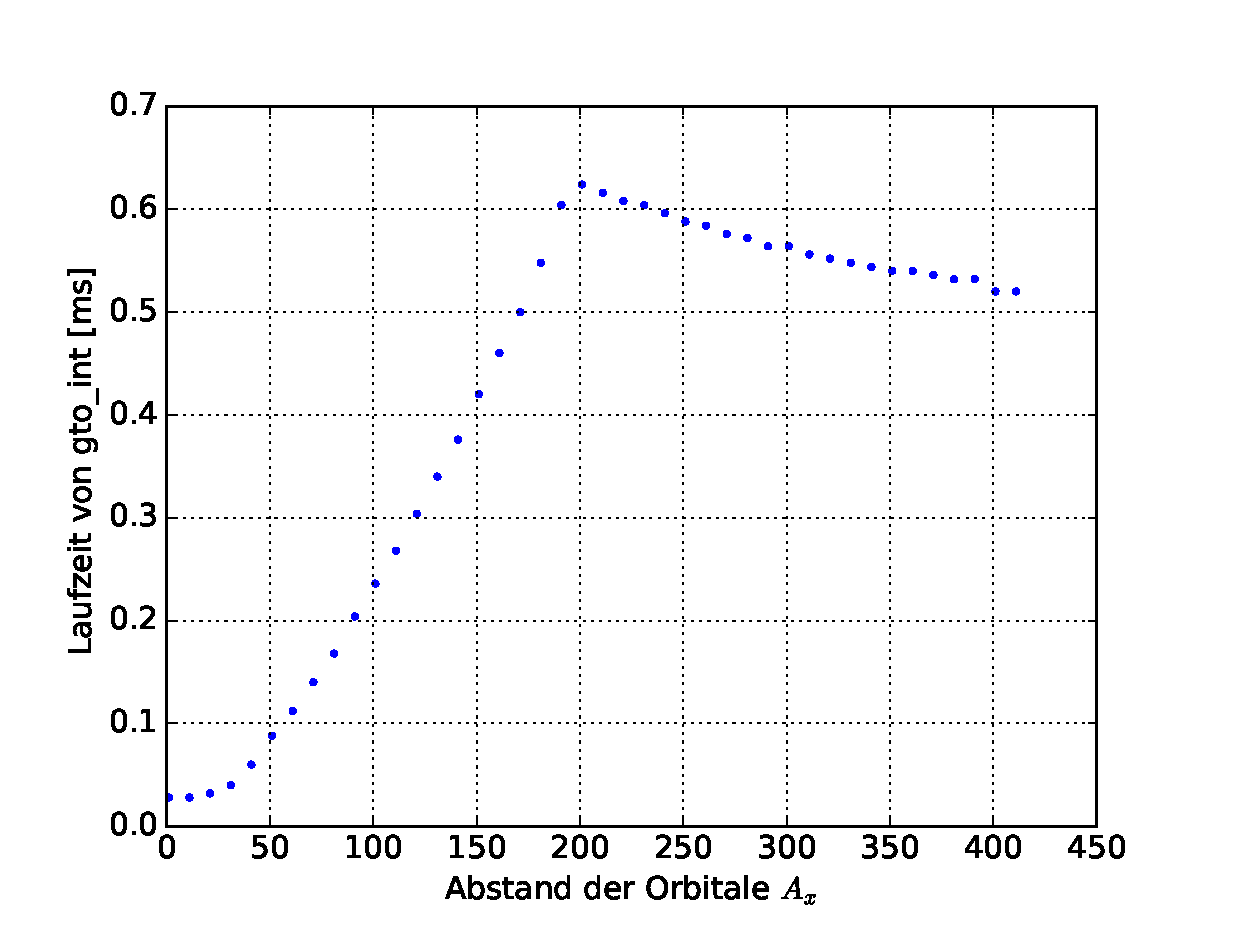
\includegraphics[scale=0.7]{Laufzeit_norm_abstand.eps}
	%\vspace*{-10mm}
	\caption{Laufzeit von \texttt{gto\_int} in Abhängigkeit des 
	Parameters $A_x$ bei der Normberechnung zu den 
	Orbitalen (0,0,1) und (0,0,0) und den Exponenten 
	a=c=0,001}
	%\vspace{2mm} %\hrule 
	\label{pic:test_norm_abstand_laufzeit} 
\end{figure}
%

%
%
%
\subsubsection{Variation des Exponenten}
%
Abschließend soll der Exponent a bzw. c variiert 
werden. Auch hier wird das (0,0,1) Orbital an 
\textbf{A}=($A_x$,0,0) in Verbindung mit dem an 
\textbf{C}=\textbf{0} 
befindlichen (0,0,0) Orbital betrachtet. Dazu muss 
zunächst ein plausibler Variationsbereich ermittelt 
werden. Das zu betrachtende physikalische Problem / 
System spielt auf zwei Größenordnungen an: zum einen auf 
der des Wechselwirkungspotentials und der des 
Fallenpotentials. Beide können in der Störungstheorie 
erster Ordnung um ihre Minima als quadratisch 
angenommen werden. Lösungen des Harmonischen Oszillators, 
Hermit-Funktionen, sind also in erster Ordnung eine 
gute Approximation der Wellenfunktionen. Dieser Sachverhalt ist in Bild 
\ref{pic:quad.naerung} dargestellt.
%
\begin{figure}[t] \centering
	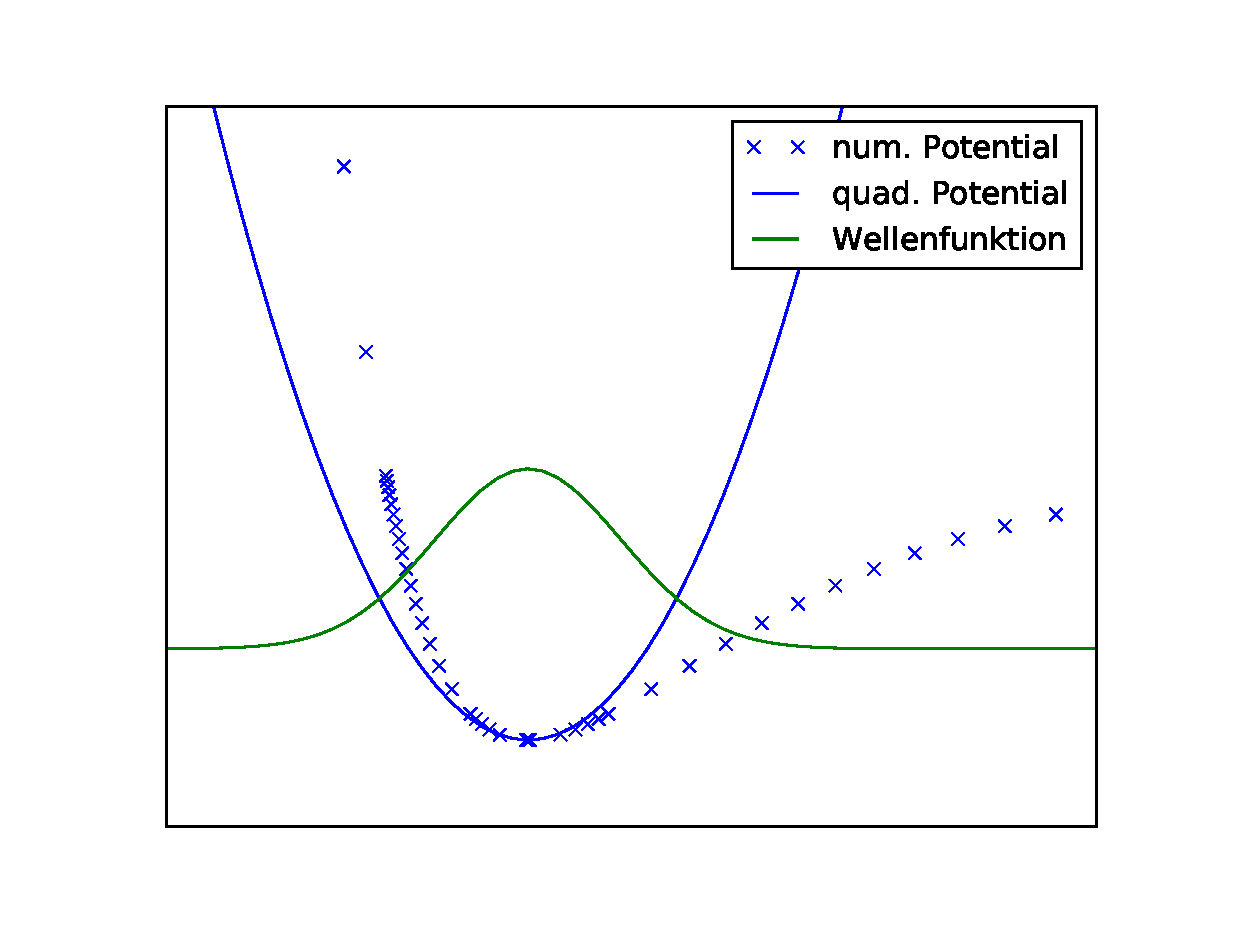
\includegraphics[scale=0.7]{HON.eps}
	\vspace*{-10mm}
	\caption{Schematische Darstellung der quadratischen Näherung und des 
	dazugehörigen Grundzustandes}
	%\vspace{2mm} %\hrule 
	\label{pic:quad.naerung} 
\end{figure}
%

Weiterhin macht diese Beobachtung zum einen die Wahl der GTOs als Ansatz sehr 
plausible, da die Hermit-(Gauß)-Funktionen in gewisser 
Weise enthalten sind und liefert auch eine Möglichkeit, 
um die Exponenten abzuschätzen. Der "Grundzustand"\ des 
als quadratisch genäherten Wechselwirkungspotentials 
kann analytisch berechnet werden. Das MRP \ref{eq:MRP} zum Beispiel nimmt in 
quadratischer 
Ordnung um das Minima\footnote{MRP stellt eine gute Beschreibung des 
numerischen Potentials um das Minima dar, vergleiche Darstellung 
\ref{pic:Pot}.} die Gestalt
%
\begin{align*}
V_\text{MRP}\approx-D_e + a_\text{st}^2\cdot D_e\cdot (r_{12}-R_m)^2 + 
\mathcal{O}(r_{12}^3) 
\end{align*}
%
an. Im Vergleich zum harmonischen Oszillator
%
\begin{align*}
V_\text{ham}=\frac12 m\omega_\text{h}^2 x^2
\end{align*}
% 
kann die Abschätzung
%
\begin{align*}
\frac12 m \omega_\text{h}^2 &= a_\text{st}^2 \cdot D_e\\
\Rightarrow \omega_\text{h}&=\sqrt{\frac{a_\text{st}^2\cdot D_e}{m}}
\end{align*}
%
gefunden werden. Aus dem Grundzustand des Harmonischen Oszillators 
%
\begin{align*}
\psi_0=\rl{\frac{m\omega_\text{h}}{\pi}}^\frac14 e^{-\frac12 m\omega_\text{h} 
x^2}
\end{align*}
%
kann nun der Exponent der Gauß-Funktion (Vergleiche \ref{pic:quad.naerung}), 
also der GTOs, 
unter Zuhilfenahme der Parameter aus Abbildung \ref{pic:Pot} und der 
Lithiummasse\footnote{$m_\text{Li}\approx12650,8 \ m_e$} in 
natürlichen Einheiten mit
%
\begin{align}
a_\text{max}\approx\frac{1}{2}a_\text{st}\sqrt{D_e\cdot m}\approx 1,074\  
a_0^{-2}
\end{align}
%
abgeschätzt werden.
Anschließend ist durch das Experiment \cite{av:7a} eine 
Frequenz für das Fallenpotential vorgegeben (siehe auch im Abschnitt 
\ref{sec:System}). 
\cite{phdthesis:sala} baut diesen Ansatz noch auf ein 
anharmonisches Potential aus, was hier noch nicht nötig 
ist. Es ergibt sich
%
\begin{align*}
a_\text{min}\approx\frac{m\omega_\text{exp}}{2}\approx2,142\cdot 10^{-9} \ 
a_0^{-2}\quad.
\end{align*}
%
Daher wird a bzw. c im Bereich von $1-10^{-10}$ 
variiert. 
%
\begin{table}[H] \centering
	\caption{Genauigkeitstest der Subroutine \texttt{gto\_int} 
		zu verschiedenen 
		Exponenten c der GTOs durch Normberechnung im Vergleich zu 
		analytischen 
		Ergebnissen mit den Konstanten a=0,001 und $A_x=1$} \vspace{0.2cm}
	\begin{threeparttable} 
		\begin{tabular}{c||c||c||c}
			c&$I_\text{gto\_int}$ & $I_\text{Norm}$ & 
			$\left|\frac{I_\text{gto\_int}-I_\text{Norm}}{I_\text{Norm}}\right|$
			 \\ \hline \hline
			1,00E+00 & 3,06407675221934E+07 & 3,06407675222225E+07 & 9,49E-13 \\
			1,00E-01 & 9,68946146259369E+08 & 9,68946146259369E+08 & 1,23E-16 \\
			1,00E-02 & 3,06407675222150E+10 & 3,06407675222225E+10 & 2,42E-13 \\
			1,00E-03 & 9,68946146260324E+11 & 9,68946146259369E+11 & 9,85E-13 \\
			1,00E-04 & 3,06407675221919E+13 & 3,06407675222225E+13 & 9,97E-13 \\
			1,00E-05 & 9,68946146259367E+14 & 9,68946146259369E+14 & 1,94E-15 \\
			1,00E-06 & 3,06407675224720E+16 & 3,06407675222225E+16 & 8,14E-12 \\
			1,00E-07 & 9,68946146163200E+17 & 9,68946146259369E+17 & 9,93E-11 \\
			1,00E-08 & 3,06407675140260E+19 & 3,06407675222225E+19 & 2,68E-10 \\
			1,00E-09 & 9,68946145997881E+20 & 9,68946146259369E+20 & 2,70E-10 \\
			1,00E-10 & 3,06407675222326E+22 & 3,06407675222225E+22 & 3,31E-13
		\end{tabular}
		%		\begin{tablenotes}
		%	\item[I] 
		%		\end{tablenotes}
	\end{threeparttable}
	\label{tab:norm:exp_c_A1}
\end{table}
%
In Tabelle \ref{tab:norm:exp_c_A1} ist zu sehen, dass das Programm über den 
gesamten Variationsbereich eine relative Abweichung von $10^{-10}$ nicht 
überschreitet. Eine leichte Tendenz zu schlechter werdenden Ergebnissen zu 
kleineren Exponenten, das heißt breiteren GTOs, ist zu erahnen. Nun soll der 
Exponent 
a variiert werden und c konstant gehalten 
werden. 
%
\begin{table}[H] \centering
	\caption{Genauigkeitstest der Subroutine \texttt{gto\_int} 
		zu verschiedenen 
		Exponenten a der GTOs durch Normberechnung im Vergleich zu 
		analytischen 
		Ergebnissen mit konstanten c=0,001 und $A_x=1$} \vspace{0.2cm}
	\begin{threeparttable} 
		\begin{tabular}{c||c||c||c}
			a&$I_\text{gto\_int}$ & $I_\text{Norm}$ & 
			$\left|\frac{I_\text{gto\_int}-I_\text{Norm}}{I_\text{Norm}}\right|$
			\\ \hline \hline
1,00E+00 & 3,06407675222224E+04 & 3,06407675222225E+04 & 2,37E-16 \\
1,00E-01 & 9,68946146259369E+06 & 9,68946146259369E+06 & 3,84E-16 \\
1,00E-02 & 3,06407675222217E+09 & 3,06407675222224E+09 & 2,30E-14 \\
1,00E-03 & 9,68946146260324E+11 & 9,68946146259369E+11 & 9,85E-13 \\
1,00E-04 & 3,06407675219172E+14 & 3,06407675222225E+14 & 9,96E-12 \\
1,00E-05 & 9,68946146259367E+16 & 9,68946146259369E+16 & 1,65E-15 \\
1,00E-06 & 3,06407677722220E+19 & 3,06407675222225E+19 & 8,16E-09 \\
1,00E-07 & 9,68945186259200E+21 & 9,68946146259369E+21 & 9,91E-07 \\
1,00E-08 & 3,06399483222180E+24 & 3,06407675222225E+24 & 2,67E-05 \\
1,00E-09 & 9,68684002260025E+26 & 9,68946146259369E+26 & 2,71E-04 \\
1,00E-10 & 3,06407675222326E+29 & 3,06407675222224E+29 & 3,32E-13 \\
1,00E-11 & 1,61319124067008E+32 & 9,68946146259369E+31 & 6,65E-01
		\end{tabular}
		%		\begin{tablenotes}
		%	\item[I] 
		%		\end{tablenotes}
	\end{threeparttable}
	\label{tab:norm:exp_a_A1}
\end{table}
%
In diesem Test ( Tabelle \ref{tab:norm:exp_a_A1} ) wird die schon oben 
beobachtete 
Tendenz zu schlechteren Ergebnissen zu kleineren Exponenten wieder beobachtet. 
Ein höheres Orbital, das heißt die höhere Komplexität, spiegelt sich damit auch 
in 
der Genauigkeit bei der Variation des Exponenten wider. Auffällig hier sind 
die Ergebnisse zu $a=\{10^{-5},10^{-10}\}$ . Hier scheinen sich numerische 
Fehler gegenseitig zu kompensieren. Weiterhin zeigt sich jetzt 
schon eine Grenzen des Programms. Für $a=10^{-11}$ fällt die Genauigkeit schon 
auf 66\% und ist damit wohl nicht mehr zweckdienlich. Dieser 
Genauigkeitsverlust entsteht vermutlich durch Verlust signifikanter Stellen bei 
einer Subtraktion zwei gleich großer Zahlen. Abschließend soll der 
letzte Test für einen anderen Abstand wiederholt werden:
 %
 \begin{table}[H] \centering
 	\caption{Genauigkeitstest der Subroutine \texttt{gto\_int} 
 		zu verschiedenen 
 		Exponenten a der GTOs durch Normberechnung im Vergleich zu 
 		analytischen 
 		Ergebnissen mit konstanten c=0,001 und $A_x=201$} \vspace{0.2cm}
 	\begin{threeparttable} 
 		\begin{tabular}{c||c||c||c}
 			a&$I_\text{gto\_int}$ & $I_\text{Norm}$ & 
 			$\left|\frac{I_\text{gto\_int}-I_\text{Norm}}{I_\text{Norm}}\right|$
 			\\ \hline \hline
1,00E+00 & 2,56024861643483E+04 & 3,06407675222225E+04 & 1,64E-01 \\
1,00E-01 & 8,24174537507960E+06 & 9,68946146259369E+06 & 1,49E-01 \\
1,00E-02 & 2,91305598288645E+09 & 3,06407675222224E+09 & 4,93E-02 \\
1,00E-03 & 9,68946146311261E+11 & 9,68946146259369E+11 & 5,36E-11 \\
1,00E-04 & 3,06407675222218E+14 & 3,06407675222225E+14 & 2,26E-14 \\
1,00E-05 & 9,68946146259371E+16 & 9,68946146259369E+16 & 1,98E-15 \\
1,00E-06 & 3,06407675222223E+19 & 3,06407675222225E+19 & 4,55E-15 \\
1,00E-07 & 9,68946146259313E+21 & 9,68946146259369E+21 & 5,80E-14 \\
1,00E-08 & 3,06407675221265E+24 & 3,06407675222225E+24 & 3,13E-12 \\
1,00E-09 & 9,68946146305179E+26 & 9,68946146259369E+26 & 4,73E-11 \\
1,00E-10 & 3,06407674635869E+29 & 3,06407675222224E+29 & 1,91E-09 \\
1,00E-11 & 9,68946146259346E+31 & 9,68946146259369E+31 & 2,40E-14 \\
1,00E-12 & 3,06407194882197E+34 & 3,06407675222225E+34 & 1,57E-06 \\
1,00E-13 & 9,68967117779157E+36 & 9,68946146259369E+36 & 2,16E-05
 		\end{tabular}
 		%		\begin{tablenotes}
 		%	\item[I] 
 		%		\end{tablenotes}
 	\end{threeparttable}
 	\label{tab:norm:exp_a_A201}
 \end{table}
 %
 Hier zeigt sich ein neuer Effekt. Für größere Abstände werden auch große 
 Exponenten ein Problem. Dieses Verhalten lässt sich wieder auf die Konvergenz 
 der 
 Reihendarstellung \ref{eq:reihe_M_kon.hyp.geo} zurückführen. An dieser 
 Stelle kann noch einmal auf die Größen \ref{eq:def:parameter y,x} hingewiesen 
 werden. y soll für eine gute Konvergenz in \ref{eq:reihe_M_kon.hyp.geo} 
 möglichst klein sein.  Ist a in der Größenordnung 1, geht y quadratisch mit 
 dem 
 Abstand. Für $A_x=201$ und a=1 ist $y\approx4\cdot10^4$, was definitiv nicht 
 mehr klein ist, wodurch das schlechte Ergebnis nicht mehr verwundert. Auf der 
 anderen Seite ist zu erkennen, dass ab a=$10^{-3}-10^{-4}$ das Ergebnis wieder 
 deutlich besser wird ($y\approx10-1$).\\
 
 Für die Tests \ref{tab:norm:exp_a_A1} und \ref{tab:norm:exp_c_A1} liegen die 
 Laufzeiten des Programms bei ungefähr 0,024 ms unabhängig vom Exponenten. Für 
 den letzten Test \ref{tab:norm:exp_a_A201} ist eine erhöhte Laufzeit für große 
 Exponenten mit 0,57 ms zu beobachten, was auf das Verhalten der 
 Reihenentwicklung zurückzuführen ist. Daraus folgert man außerdem, dass der 
 Genauigkeitsverlust für sehr kleine Exponenten nicht an der Reihendarstellung, 
 sondern an anderen Programmteilen liegt, wie oben schon vermutet.\\% 
 %Vorstellbar ist hier wieder der 
 %Verlust von signifikanten Stellen durch Subtraktion zweier Gleichgroßer 
 %Zahlen, wie z.B. in Formel \ref{eq:S,alpha>0}. \\
 
 Zusammenfassend kann gesagt werden, dass das Programm für niedrige Orbitale 
 und für kleine y, das heißt kleine Abstände und moderate Exponenten, eine 
 hinreichend gute relative Genauigkeit von mindestens $10^{-10}$ erreicht. Die 
 Laufzeiten sind für die gut zu bestimmbaren Integralen unter 1 ms und abhängig 
 vom Abstand noch deutlich geringer. 
%
%
%
\subsection{Reguläres Wechselwirkungspotential 
($f_{12}=r_{12}^2$)}\label{sec:T:quad}
%
Nachdem im letzten Abschnitt gezeigt wird, dass das Programm für ein neutrales 
Wechselwirkungspotential prinzipiell funktioniert, soll nun ein einfaches, 
nicht divergentes Wechselwirkungspotential getestet werden. Hier soll nun 
geprüft werden, ob das Programm auch mit einer Mischung der Koordinaten 
zurechtkommt und ob der Einfluss einer Wechselwirkung die Genauigkeit 
beeinflusst.  
Eine Problematik hierbei ist, dass nun das Integral nicht mehr mit Normen 
berechnet werden kann. Daher wird mit der numerischen Berechnung der 
NAG-Routine die Genauigkeit überprüft. \\
Auch hier sollen, um die Parameter übersichtlich zu halten, die Annahmen 
\ref{eq:tests:annahmen:norm} gelten.
Das Integral nimmt mit dem quadratischen Wechselwirkungspotential 
$f_{12}=V_2=r_{12}^2$
\ref{eq:def:V2} die Form
%
\begin{align*}
 I=\int\ d\textbf{r}_1 d\textbf{r}_2\   \cdot 
 x_{1,A}^{2i}\,y_{1,A}^{2k}\,z_{1,A}^{2m}\cdot e^{-2ar_{1,A}^2} \cdot r_{12}^2 
 \cdot x_{2,C}^{2i'}\,y_{2,C}^{2k'}\,z_{2,C}^{2m'} \cdot  e^{-2c 
 r_{2,C}^2}
\end{align*}
%
an. 
%
%
%
\subsubsection{Variation des Orbitals}
%
Zunächst wird analog zur Normberechnung die Abhängigkeit der Genauigkeit zur 
Wahl des Orbitals getestet. $(i',k',m')$ sei wieder $(0,0,0)$ und 
$(i,k,m)$ 
eine Variation.
%
 \begin{table}[H] \centering
 	\caption{Genauigkeitstest der Subroutine \texttt{gto\_int} 
 		zu verschiedenen 
 		Exponenten a der GTOs zu einem quadratischen Wechselwirkungspotential 
 		im Vergleich zu numerischen NAG-Routine mit konstanten c=0,001 und 
 		$A_x=1$} \vspace{0.2cm}
 	\begin{threeparttable} 
 		\begin{tabular}{c||c|c|c||c}
 Orbital & $I_\text{gto\_int}$ & $I_\text{NAG}$& ACC [\%] & 	
 $\left|\frac{I_\text{gto\_int}-I_\text{NAG}}{I_\text{gto\_int}}\right|$
 \\ \hline\hline
(0,0,0)&3,87578458503748E+09 & 3,8757822000E+09 & 6,73E-05 & 6,15E-07 \\
(0,0,1)&9,68946146259370E+11 & 9,6893670144E+11 & 1,02E-04 & 9,75E-06 \\
(0,0,2)&7,26709609873341E+14 & 7,2670802178E+14 & 9,03E-05 & 2,19E-06 \\
(1,0,0)&9,68946146260324E+11 & 9,6894050977E+11 & 1,07E-04 & 5,82E-06 \\
(1,0,1)&2,42236536624686E+14 & 2,4223431793E+14 & 1,71E-04 & 9,16E-06 \\
(1,2,0)&1,81677760185790E+17 & 1,8167479946E+17 & 1,44E-04 & 1,63E-05 \\
(2,0,0)&7,26709611782121E+14 & 7,2642851744E+14 & 8,18E-05 & 3,87E-04 \\
(2,0,1)&1,81678118290674E+17 & 1,8137431973E+17 & 1,28E-04 & 1,67E-03
 		\end{tabular}
 		%		\begin{tablenotes}
 		%	\item[I] 
 		%		\end{tablenotes}
 	\end{threeparttable}
 	\label{tab:r2_orbit}
 \end{table}
%
Wie in Tabelle \ref{tab:r2_orbit} zu sehen, liefert \texttt{gto\_int} 
vergleichbare, 
wahrscheinlich bessere Ergebnisse als die NAG-Routine für kleine Orbitale. Die 
wahre Genauigkeit kann hier nicht abgeschätzt werden, da die NAG-Routine auf 
ungefähr $10^{-4}-10^{-5}$ beschränkt ist. Im Vergleich zur Normberechnung 
stellt man 
jedoch fest, dass schon das (2,0,1) Orbital deutlich schlechter geworden ist. 
Weiterhin stellt man fest, dass das Integral des (2,0,0) Orbitals wesentlich 
schlechter als das Integral des (0,0,2) Orbitals berechnet wird. Anscheinend 
ist also die Genauigkeit durch die Potenz in Richtung des Abstandes  
beeinflusst und nun nicht mehr für alle Orbitale des selben l gleich. %TODO 
%LAUFZEIT fatzit 
%
%
%
\subsubsection{Variation des Abstands}
%
Nun soll der Abstandsparameter $A_x$ variiert werden. Grafik 
\ref{pic:quad.WW_Abstand} zeigt die Integralwerte der \texttt{gto\_int} Routine 
im 
Vergleich zur NAG-Routine und einer quadratischen Funktion.
%
\begin{figure}[H] \centering
	\subfigure[]{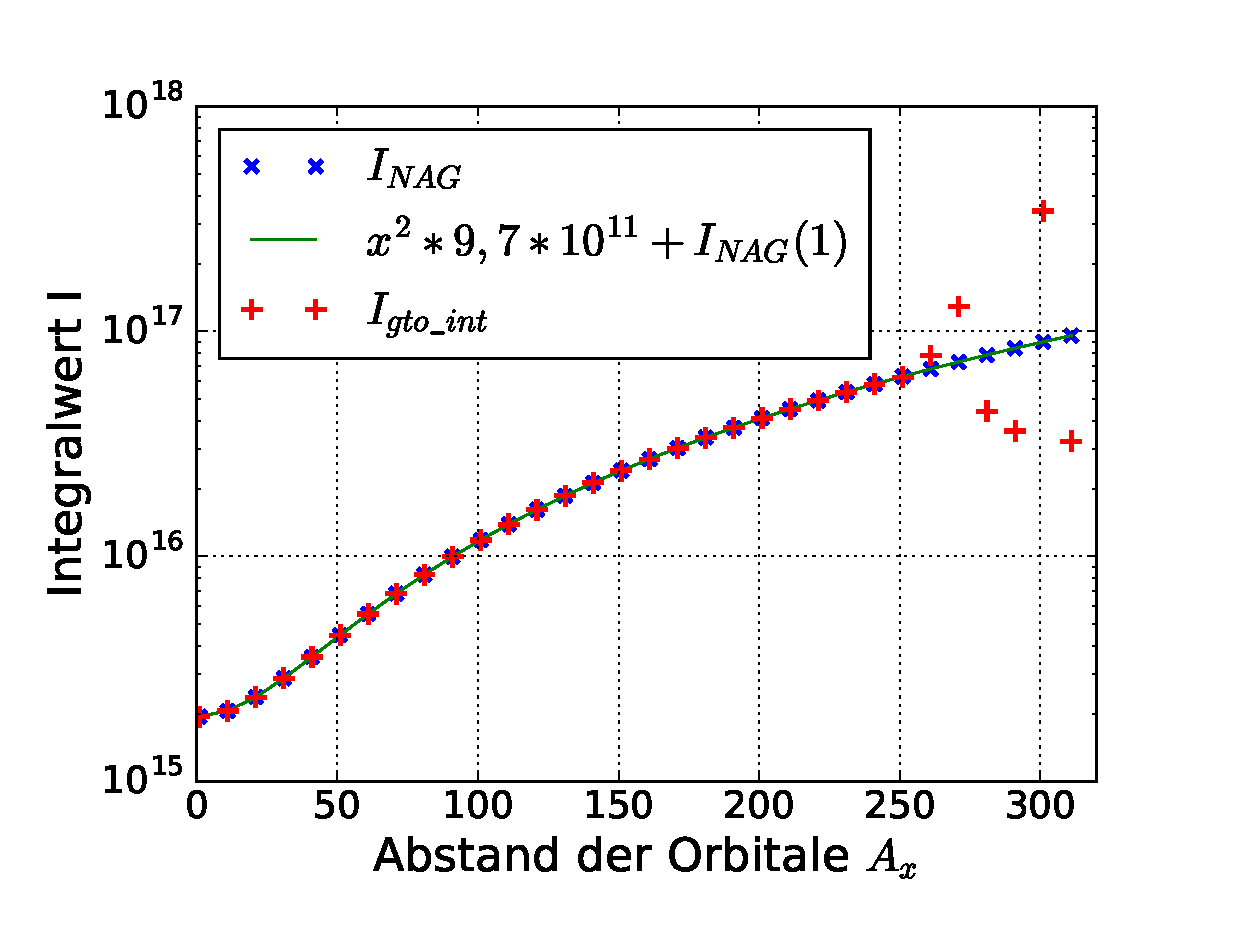
\includegraphics[scale=0.55]{r2_1.eps}} %0.35
	\subfigure[]{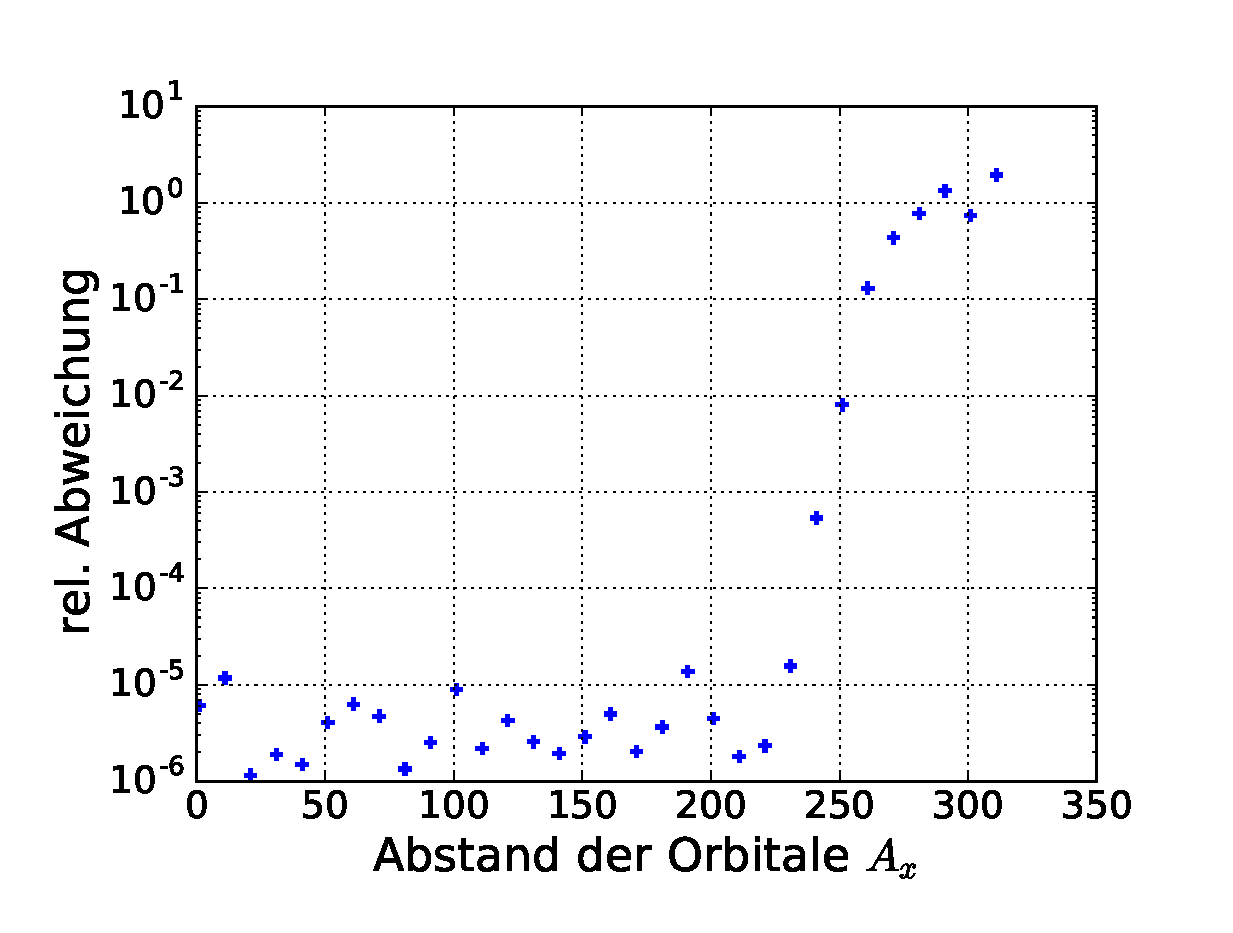
\includegraphics[scale=0.55]{r2_2.eps}}
	%\vspace*{-10mm}
	\caption{(a) Vergleich der Ergebnisse der \texttt{gto\_int} und der 
	NAG-Routine zu 
	verschiedenen Werten des Abstandsparameters $A_x$, wobei die Orbitale 
	(1,0,0) mit dem Exponenten a=0,001 und (0,0,0) mit dem Exponenten c=0,001 
	betrachtet worden sind. 	Zusätzlich ist eine quadratische Funktion 
	dargestellt. 
	(b)  zeigt die relative Abweichung zwischen $I_\text{NAG}$ und 
	$I_\text{gto\_int}$ .  } 
	%\vspace{2mm} %\hrule 
	\label{pic:quad.WW_Abstand}
\end{figure}
%
Vergleichbar zum analogen Test bei der Normberechnung sieht man in Grafik 
\ref{pic:quad.WW_Abstand} (b) , dass \texttt{gto\_int} für $A_x$ größer als 
rund 
230 einen immer größer werdenden Genauigkeitsverlust hat. Vergleicht man mit 
der 
Tabelle \ref{tab:norm:abstand_2} im Anhang \ref{sec:AnhangC:Tests}, so kann  
festgestellt werden, dass auch dort für $A_x$ größer als 230 die Genauigkeit 
schlechter als $10^{-5}$ wird. Daher scheinen für die Variation des Abstandes 
eines gegebenen Orbitals, keine neuen Verluste aufzutreten. Der rapide 
Genauigkeitsverlust kann analog zur Normberechnung auf die Reihendarstellung 
\ref{eq:reihe_M_kon.hyp.geo} zurückgeführt werden. Die Laufzeit hat auch die in 
Grafik \ref{pic:test_norm_abstand_laufzeit} dargestellten Verlauf und befindet 
sich in der selben Größenordnung. \\
In Abbildung \ref{pic:quad.WW_Abstand} (a) ist zu erkennen, dass 
$I_\text{gto\_int}$ den numerischen Ergebnissen $I_\text{NAG}$ weitgehend 
folgt. Zusätzlich kann man feststellen, dass bei Verwendung einer quadratischen 
Wechselwirkung die Integralwerte entsprechend eines quadratischen Verlaufs bei 
der Variation des Abstandes zeigen, was durch die hinzugefügte Funktion 
ersichtlich ist. Die Integralwerte fächern bei steigender Ungenauigkeit um das 
richtige Ergebnis auf.    
%
%
%
\subsubsection{Variation des Exponenten}
%
Bei der Variation des Exponenten ist analog zur Normberechnung vorgegangen 
worden, das heißt, die Tests werden unter den gleichen Annahmen und mit den 
selben 
Werten der konstanten Parameter durchgeführt. Dabei ist ein immer gleiches 
Verhalten beobachtet worden. 
%
\begin{figure}[H] \centering
	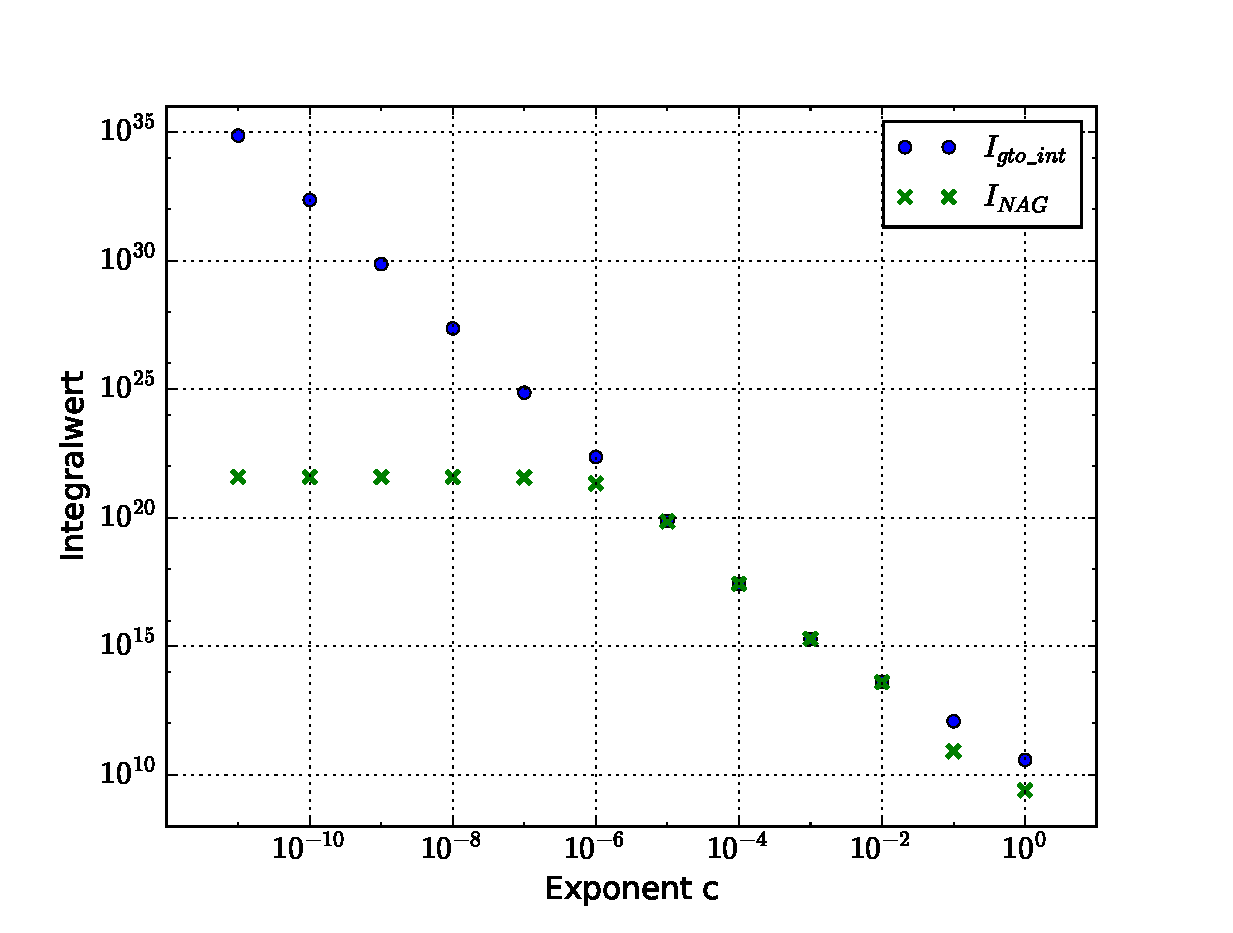
\includegraphics[scale=0.7]{r2_3.eps}
	%\vspace*{-10mm}
	\caption{Vergleich der Ergebnisse der \texttt{gto\_int} und der NAG-Routine 
	zu unterschiedlichen Exponenten c bei a=0,001 , $A_x=101$ und 
	\textbf{C}=\textbf{0}.}
	%\vspace{2mm} %\hrule 
	\label{pic:quad.WW_exponent} 
\end{figure}
%
Wie in Abbildung \ref{pic:quad.WW_exponent} zu sehen ist, gibt es zwei Bereiche,
in denen \texttt{gto\_int} von der NAG-Routine abweicht und einen Bereich 
($10^{-2}-10^{-5}$), indem sie folgt. Im Letzteren beträgt die Abweichung 
ungefähr $10^{-6}$; wie oben schon gesehen, stimmt in dem Bereich also 
\texttt{gto\_int} so gut es nur geht mit $I_\text{NAG}$ überein. Für große 
Exponenten tritt wieder die oben beschriebene Abweichung aufgrund der 
Reihendarstellung im Basisintegral ein. Die auftretende Abweichung für 
Exponenten kleiner als $10^{-5}$ ist ein technisches Problem. Bei der 
Verwendung der NAG-Routine muss ein endliches Berechnungsintervall gegeben 
werden. Da für kleine Exponenten die GTOs aber immer breiter werden, wird 
irgendwann das gesamte Intervall von der GTO ausgefüllt und es wird quasi über 
eine Waagerechte integriert (Rechteck). Daher nimmt $I_\text{NAG}$ einen 
maximalen Wert an für kleiner werdende Exponenten. Es wird versucht, 
entsprechend das Intervall auf eine andere Größenordnung mit zu skalieren, 
jedoch scheint die NAG-Routine intern Abtastalgorithmen zu verwenden, die dann 
keine veränderliche Funktion mehr wahrnimmt, frühzeitig abbricht und 0 als 
Ergebnis ausgibt. Analog sei erwähnt, dass auch die Abweichung für große 
Exponenten prinzipiell durch Fehler beim Abtasten in der NAG-Routine 
entstanden sein kann.   %\\%letztes ist seh wichtig !!
Weiterhin ist in \ref{pic:quad.WW_exponent} zu erkennen, dass der prinzipielle 
Verlauf der Integralwerte von $I_\text{NAG}$ im Übereinstimmungsbereich weiter 
gefolgt wird. Das ist ein Indiz dafür, dass  $I_\text{gto\_int}$ auch für 
kleinere Exponenten plausible Werte liefert. Hinzu kommt, dass auch noch kein 
Auffächern oder ähnliche extreme Schwankungen zu erkennen sind.
%
%
%
\subsection{Renormierungsschema}
%
In \texttt{int\_S\_sub} wird innerhalb der T-Blöcke ein Renormierunsschema 
verwendet. Dieses ist im Abschnitt \ref{sec:renorm} erklärt. Auf Grund der 
Renormierung können solche Integrale nicht mit einer numerischen Routine 
überprüft werden. Daher wird die Untersuchung der Plausibilität der 
Integralwerte nicht mehr in dieser Arbeit erörtert. Die Lösung (das 
Energiespektrum) für das 
Zweiteilchenproblem $^7$Li$^7$Li ist in \cite{phdthesis:sergey} gegeben, 
daher kann das Renormierungsschema an diesem physikalischen Beispiel getestet 
und geprüft werden, was auch nicht mehr in dieser Arbeit geschieht. Im Vorfeld 
kann jedoch noch eine Konsistenzprüfung durchgeführt werden. Zur Erinnerung es 
geht um Integrale des Typs \ref{eq:def:T-Int} :
%
\begin{align*}
T_s^\pm(x)&:=\mathcal{R}\int_{0}^{\infty}\frac{dz}{z^s}e^{\pm z-xz^2} \quad.
\end{align*}
%
Zur Berechnung dieser ist im Abschnitt \ref{sec:renorm} erklärt, dass die 
Rekursion \ref{eq:recursivT} für $x=\frac{\gamma}{\beta^2}>1$ und die Rekursion 
\ref{recursiveT2} für x<1 verwendet werden soll, wobei $\gamma$ und 
$\beta$ potentialspezifische Parameter sind.  \ref{eq:recursivT} 
 startet mit berechenbaren Integralen. $\omega_1(x)$ und $\omega_0(x)$ sind 
 durch numerische Integration im Rahmen der in \cite{av:1a2} angegebenen 
 Grenzen überprüft worden. Auf Tipp- und Logikfehler ist durch eine unabhängige 
 MATHEMATICA-Implementierung getestet worden. Dabei sind für \ref{eq:recursivT} 
 keine Anomalien aufgetreten. Bei der Berechnung der Rekursion 
 \ref{recursiveT2} (fallender Index) hingegen ist aufgefallen, dass $T_s$ nicht 
 unabhängig von dem gewählten oberen Startindex $s_\text{max}$ ist. Abbildung 
 \ref{pic:Trec} zeigt das Verhalten an 3 repräsentativen Beispielen für 
 verschiedene x.    
%
\begin{figure}[t] \centering
	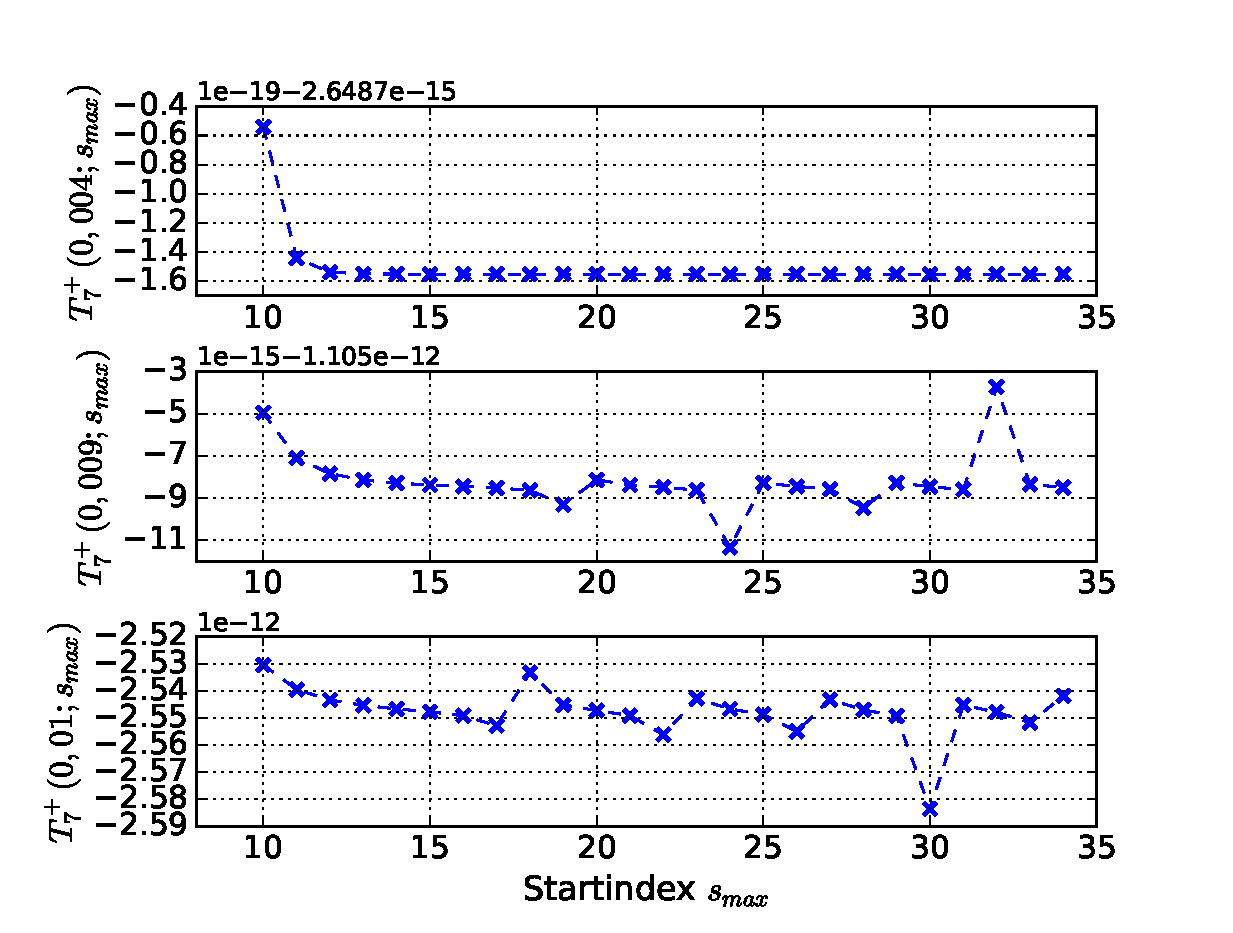
\includegraphics[scale=0.7]{Trec.eps}
	%\vspace*{-10mm}
	\caption{Konvergenzverhalten der Rekursion \ref{recursiveT2} zur Berechnung 
	von $T^+_s(x)$ für 
	verschiedene Startindizes $s_\text{max}$ am Beispiel s=7 und x=$\{0,004 ,\ 
	0,009 ,\ 0,01 \}$ }
	%\vspace{2mm} %\hrule 
	\label{pic:Trec} 
\end{figure}
%

Zu erwarten wäre ein Annähern der Integralwerte an eine 
Konstante, sodass es ein fixes $s_\text{max}$ gibt, ab dem die Rekursion 
unabhängig von $s_\text{max}$ wird. 
Zunächst ist zu sagen, dass die FORTRAN Implementierung bei x<0,004 als 
Ergebnis 0 ausgibt. Zumal kann $T_0^+$ hier schon auf Grund des 
Exponentialfaktors $e^{\frac{1}{4x}}$ den Darstellungsbereich 
\texttt{real(KIND=8)} (double percision) verlassen und so bei der 
Nachskalierung einen undefinierten Wert ergeben. Weiterhin kann es dazu kommen, 
dass z.B. $T_0^-$ auf exakt 0 gerundet wird, da die \texttt{Erf}-Funktion schon 
auf exakt 1 gerundet wird. \\
Im obersten Bild der Grafik \ref{pic:Trec} ist zu erkennen, dass hier das 
beschriebene Vorgehen aus Abschnitt \ref{sec:renorm} äußerst gut funktioniert. 
Es wird ab $s_\text{max}=28$ ein auf 16 signifikante Stellen konstantes 
Ergebnis berechnet\footnote{Alle Berechnungen sind bis $s_\text{max}=100$ 
durchgeführt worden, jedoch nur bis $s_\text{max}=34$ dargestellt.}. Im 
mittleren und unteren Bild ist jedoch zu erkennen, dass die Rekursion abhängig 
von $s_\text{max}$ nicht auf die gewünschte Genauigkeit konvergiert. Für kleine 
Startindizes ist das erwartete Annähern an das Ergebnis zu beobachten, jedoch 
schlägt z.B. im mittleren Bild bei $s_\text{max}=19$ die Kurve aus. 
Anschließend scheint wieder eine Annäherung zu entstehen, welche durch einen 
weiteren Ausschlag bei 24 unterbrochen wird. Die Schwankungen liegen im 
mittleren Bild im Bereich von 0,1\%. Ein analoges Verhalten ist auch in 
untersten Bild in \ref{pic:Trec} zu sehen. Hier liegt die Schwankung jedoch in 
Bereich von 10\%. Die Tendenz, dass pro 0,001 Schritt in x 2-3 Größenordnungen 
der Genauigkeit verloren geht, ist auch für 0,004<x<0,009 und für x>0,01 zu 
sehen. Im letzteren Fall hat man also keine signifikanten Stellen des 
Ergebnisses mehr, lediglich eine Größenordnung. Für größere x sind die 
Sprungstellen und die abschnittsweise Annäherung an das Ergebnis, analog zur 
Abbildung \ref{pic:Trec}, deutlicher zu sehen.  Es stellt sich nun die Frage ob 
die Verwendung in einem so eingeschränkten Anwendungsbereich noch Sinn macht. 
Um die Genauigkeit zu verbessern, kann versucht werden die Rekursion 
\ref{recursiveT2} auf einem höheren Datentyp (z.B. \texttt{real(KIND=16)}) 
ablaufen zu lassen, da Verlust signifikante Stellen durch Subtraktion zweier 
gleich großer Zahlen entstehen kann.
%
%
%
%\subsection{Zusammenfassung}
%
%Im Rahmen der hier dargestellten Tests ist festgestellt worden, dass 
%\texttt{gto\_int} für niedrige Orbitale, das heißt l<6 ,effektive Abstände 
%Q<200 und für große Bereiche der Exponenten a/c eine relative Genauigkeit von 
%ungefähr $10^{-10}$ erreichen kann. Der limitierende Faktor bzgl. des 
%Abstandes 
%stellt die Reihendarstellung \ref{eq:reihe_M_kon.hyp.geo} und damit die 
%Berechnung des Basisintegrals dar. Die Größe y sollte dabei möglichst kleiner 
%als 1 sein. Für höhere Orbitale und Exponenten kleiner als $10^{-10}$ sind 
%andere Effekte verantwortlich. Zu vermuten ist, dass bei einer Subtraktion 
%zweier gleichgroßer Zahlen signifikante Stellen verloren gehen.
% 
%
%
\section{Optimierungsvorschläge}
%
In diesem Projekt wird in erster Linie darauf hin gearbeitet, das Programm 
\texttt{gto\_int} bzw. \texttt{gto\_int\_test} und damit den Algorithmus zum 
Laufen zu bringen. Hierbei wird aus Zeitgründen und der Einfachheit halber 
einige Kompromisse bzgl. der Programmoptimierung getroffen. Im Folgenden werden 
schon bekannte, aber noch nicht implementierte Optimierungen des Quellcodes 
vorgeschlagen.
\begin{enumerate}
	\item Es soll eine andere Berechnungsmethode des Basisintegrals 
	gefunden und implementiert werden. Dazu bietet sich an, den in 
	\cite{av:1a} / \cite{av:1a2} vorgestellten Weg zu wählen, jedoch muss 
	dazu 
	erst der Fehler in Gleichung (60) aus \cite{av:1a} berichtigt und auf 
	alle darauf folgenden Gleichungen angewandt werden, erste Ansätze sind 
	dafür schon vorhanden.
	%
	\item Im Programmabschnitt \texttt{sum\_R\_sum} werden die soliden reellen 
	Kugelflächenfunktionen Z als Funktion von sin und cos Funktionen 
	aufgerufen. Da der Vektor \textbf{Q} und damit deren Polardarstellung schon 
	kurz nach Aufruf der \texttt{gto\_int} Routine bekannt ist, soll schon dort 
	der sin und cos Wert ausgewertet und gespeichert werden. So kann eine 
	ganze Reihe an Funktionsaufrufen, die in Reihenentwicklungen enden, 
	eingespart werden. Weiterhin kann so Z schon als Matrix oder besser Vektor 
	vor den äußeren Schleifen in \ref{pic:FC:sum_R_sub} berechnet werden; dies 
	spart wiederum Laufzeit und Speicherplatz.
	%
	\item Der Koeffizient $c^{-1}$ in \texttt{sum\_R\_sub} wird über Aufrufe 
	der Schlegel-Koeffizienten c berechnet. Dabei wird aktuell c noch als 
	Funktion gehandhabt. Sowohl c als auch $c^{-1}$ können, da sie von keinen 
	fallspezifischen Parametern abhängen, einmalig für einen großen Bereich 
	der Indizes, berechnet und auf der Festplatte gespeichert werden. Dabei 
	soll weiterhin eine Vektorisierung des noch 5-d-Feldes vorgenommen werden. 
	Diese Optimierung 	spart Rechenzeit, da weniger Funktionsaufrufe und 
	keine Berechnungsschleifen mehr notwendig sind. Weiterhin spart man dabei 
	Speicherplatz, da durch eine Vektorisierung keine nicht genutzten Nullen 
	mehr gespeichert werden müssten.
	%
	\item Der Koeffizient d in \texttt{sum\_R\_sub} wird innerhalb von einer 
	Schleife berechnet, das heißt, \texttt{d\_coef} wird dort erst aufgerufen. 
	Es soll \texttt{d\_coef} so	angepasst werden, sodass der Aufruf schon 
	außerhalb der Schleife geschehen kann. Weiterhin  ist d auch unabhängig von 
	fallspezifischen Parametern, das heißt,	auch d kann einmal vorberechnet 
	und anschließend auf der Festplatte gespeichert werden. Diese 
	können dann für alle folgenden Integrale abgerufen werden. Außerdem soll 
	auch d als Vektor gespeichert werden, um die Laufzeit weiter zu optimieren 
	und unnötige Nullen nicht zu speichern.
    % 
\end{enumerate} 
%
%
%